This chapter presents the simulation study results.

\section{SIMULATION STUDY}
\label{cap:simures}

\newpage
\begin{figure}[H]
 \setlength{\abovecaptionskip}{.0001pt}
 \caption{PARAMETER BIAS WITH 2.5\% AND 97.5\% QUANTILES}
 \vspace{0.2cm}\centering
 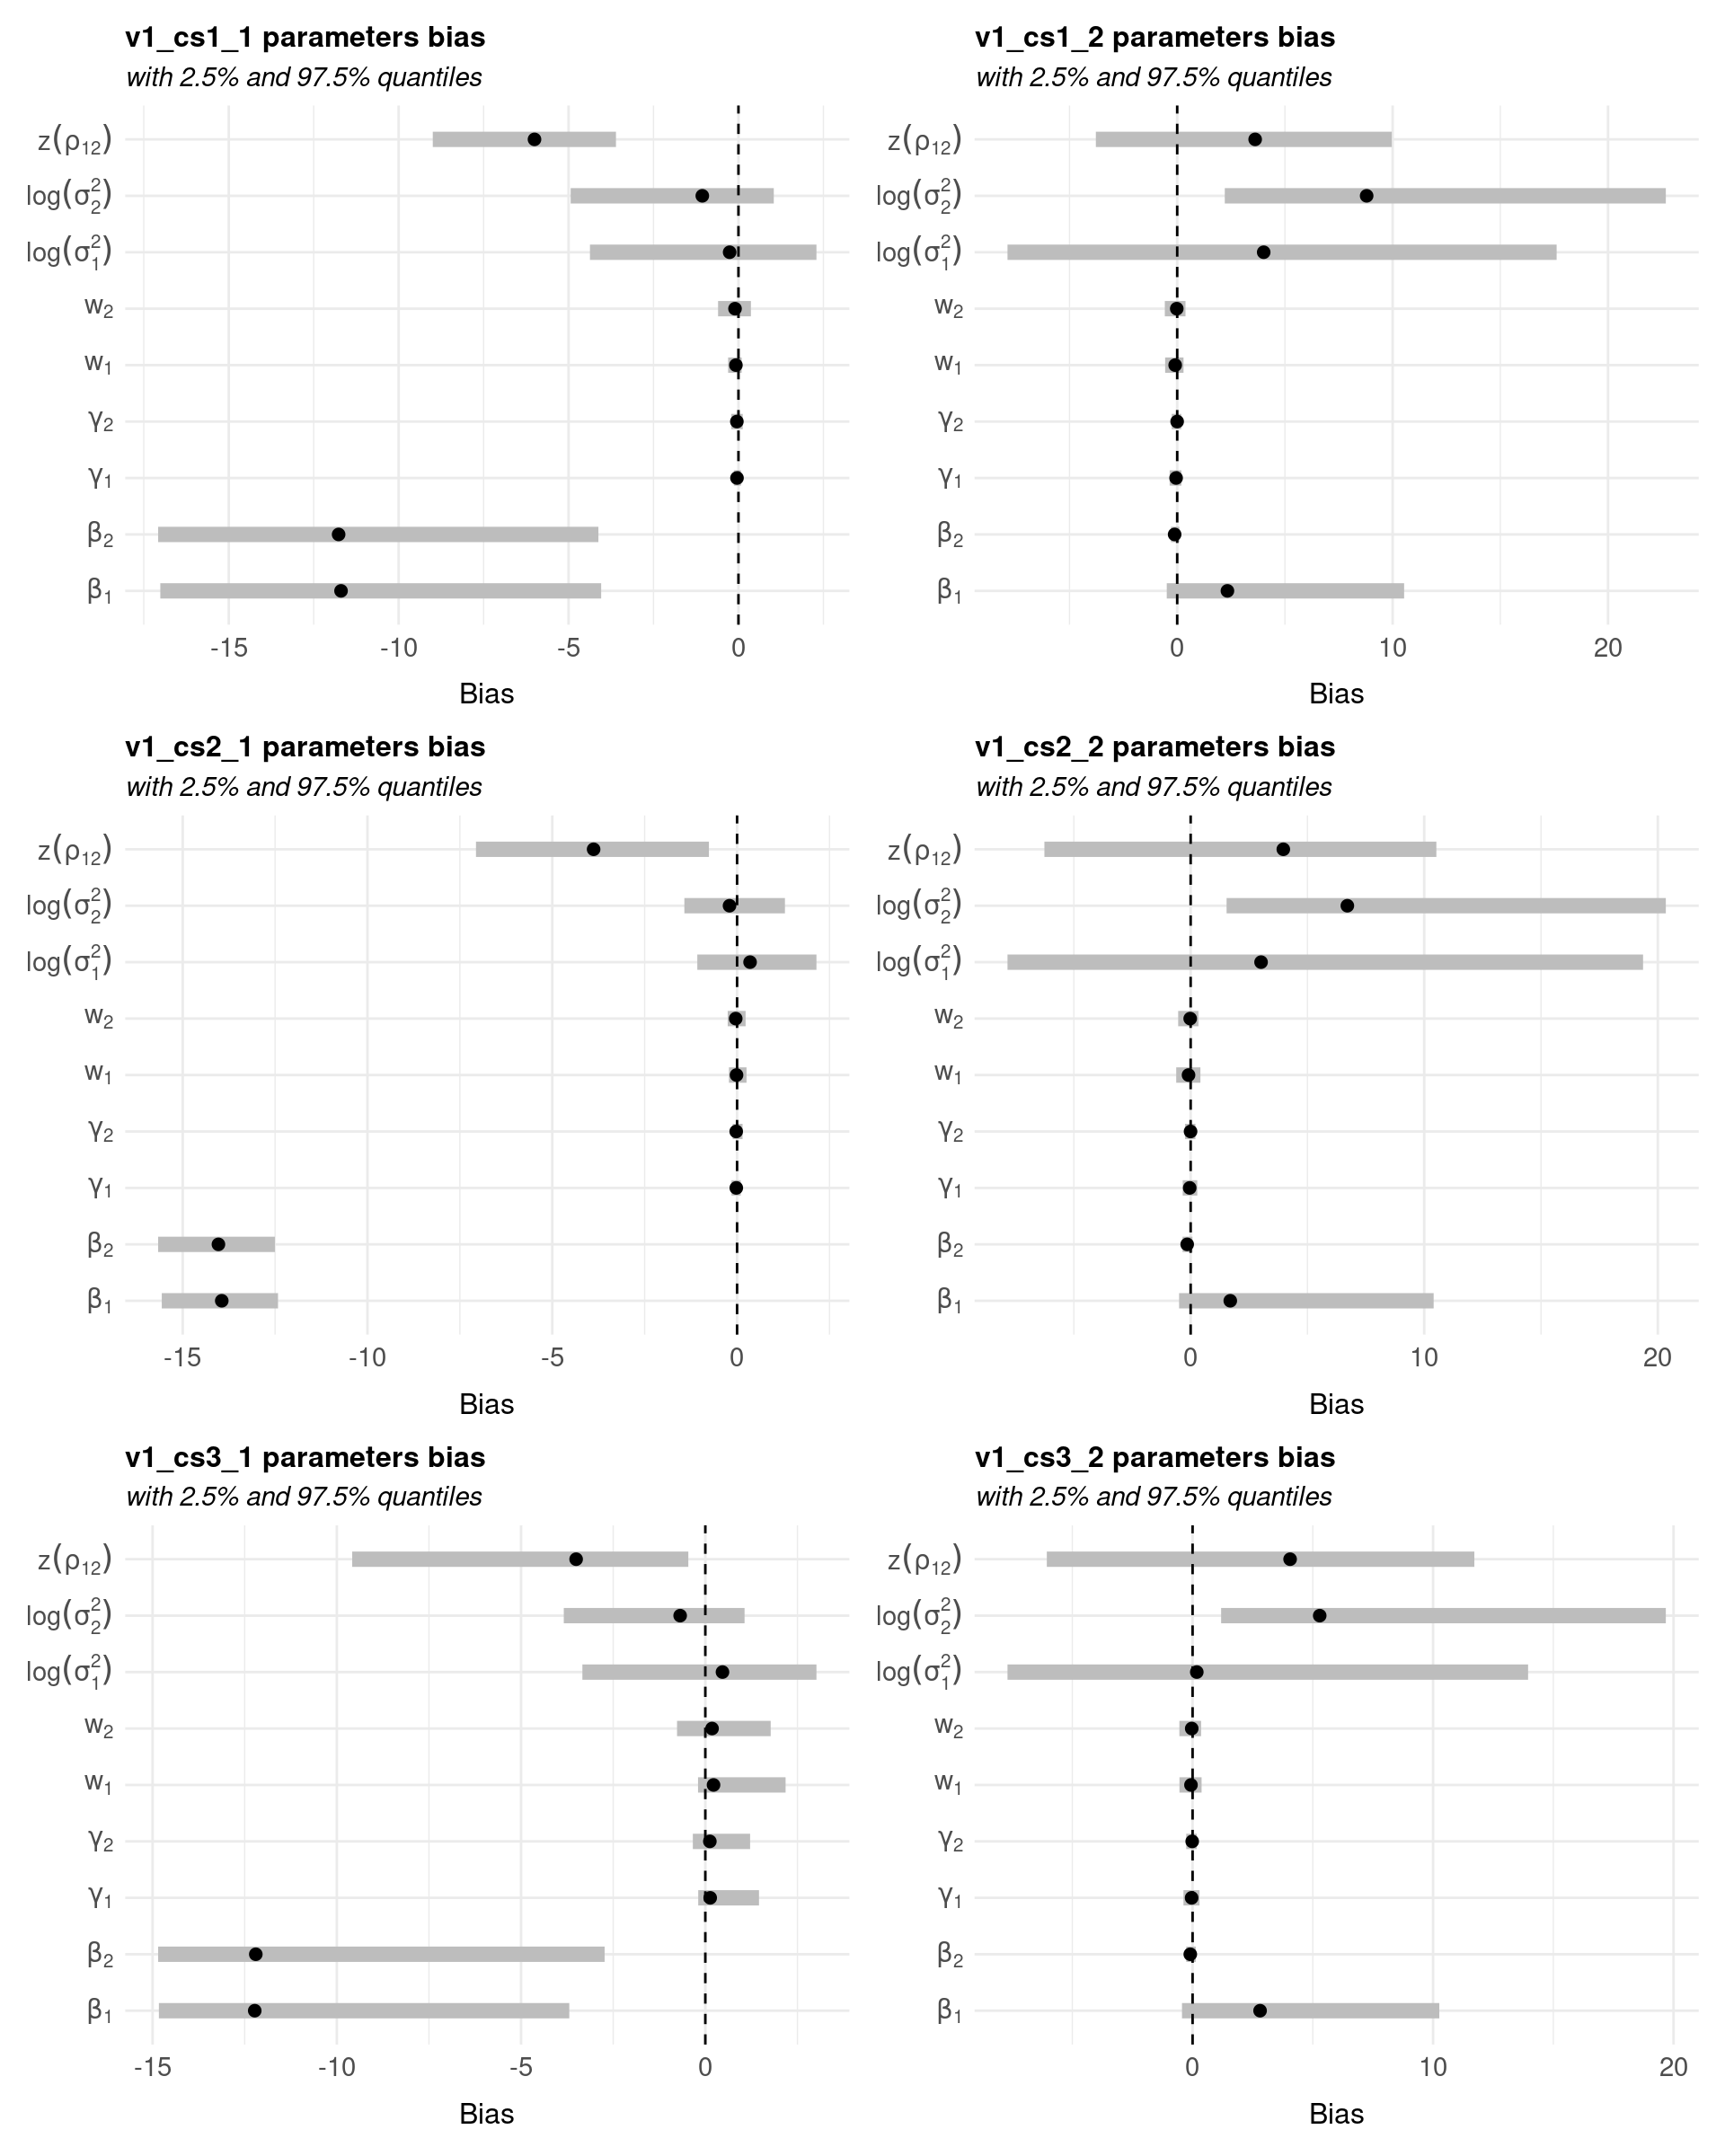
\includegraphics[width=\textwidth]{bias2plot-1.png}\\
 \begin{footnotesize}
  SOURCE: The author (2021).
 \end{footnotesize}
 \label{fig:biasbeta1}
\end{figure}

\begin{figure}[H]
 \setlength{\abovecaptionskip}{.0001pt}
 \caption{PARAMETER BIAS WITH 2.5\% AND 97.5\% QUANTILES}
 \vspace{0.2cm}\centering
 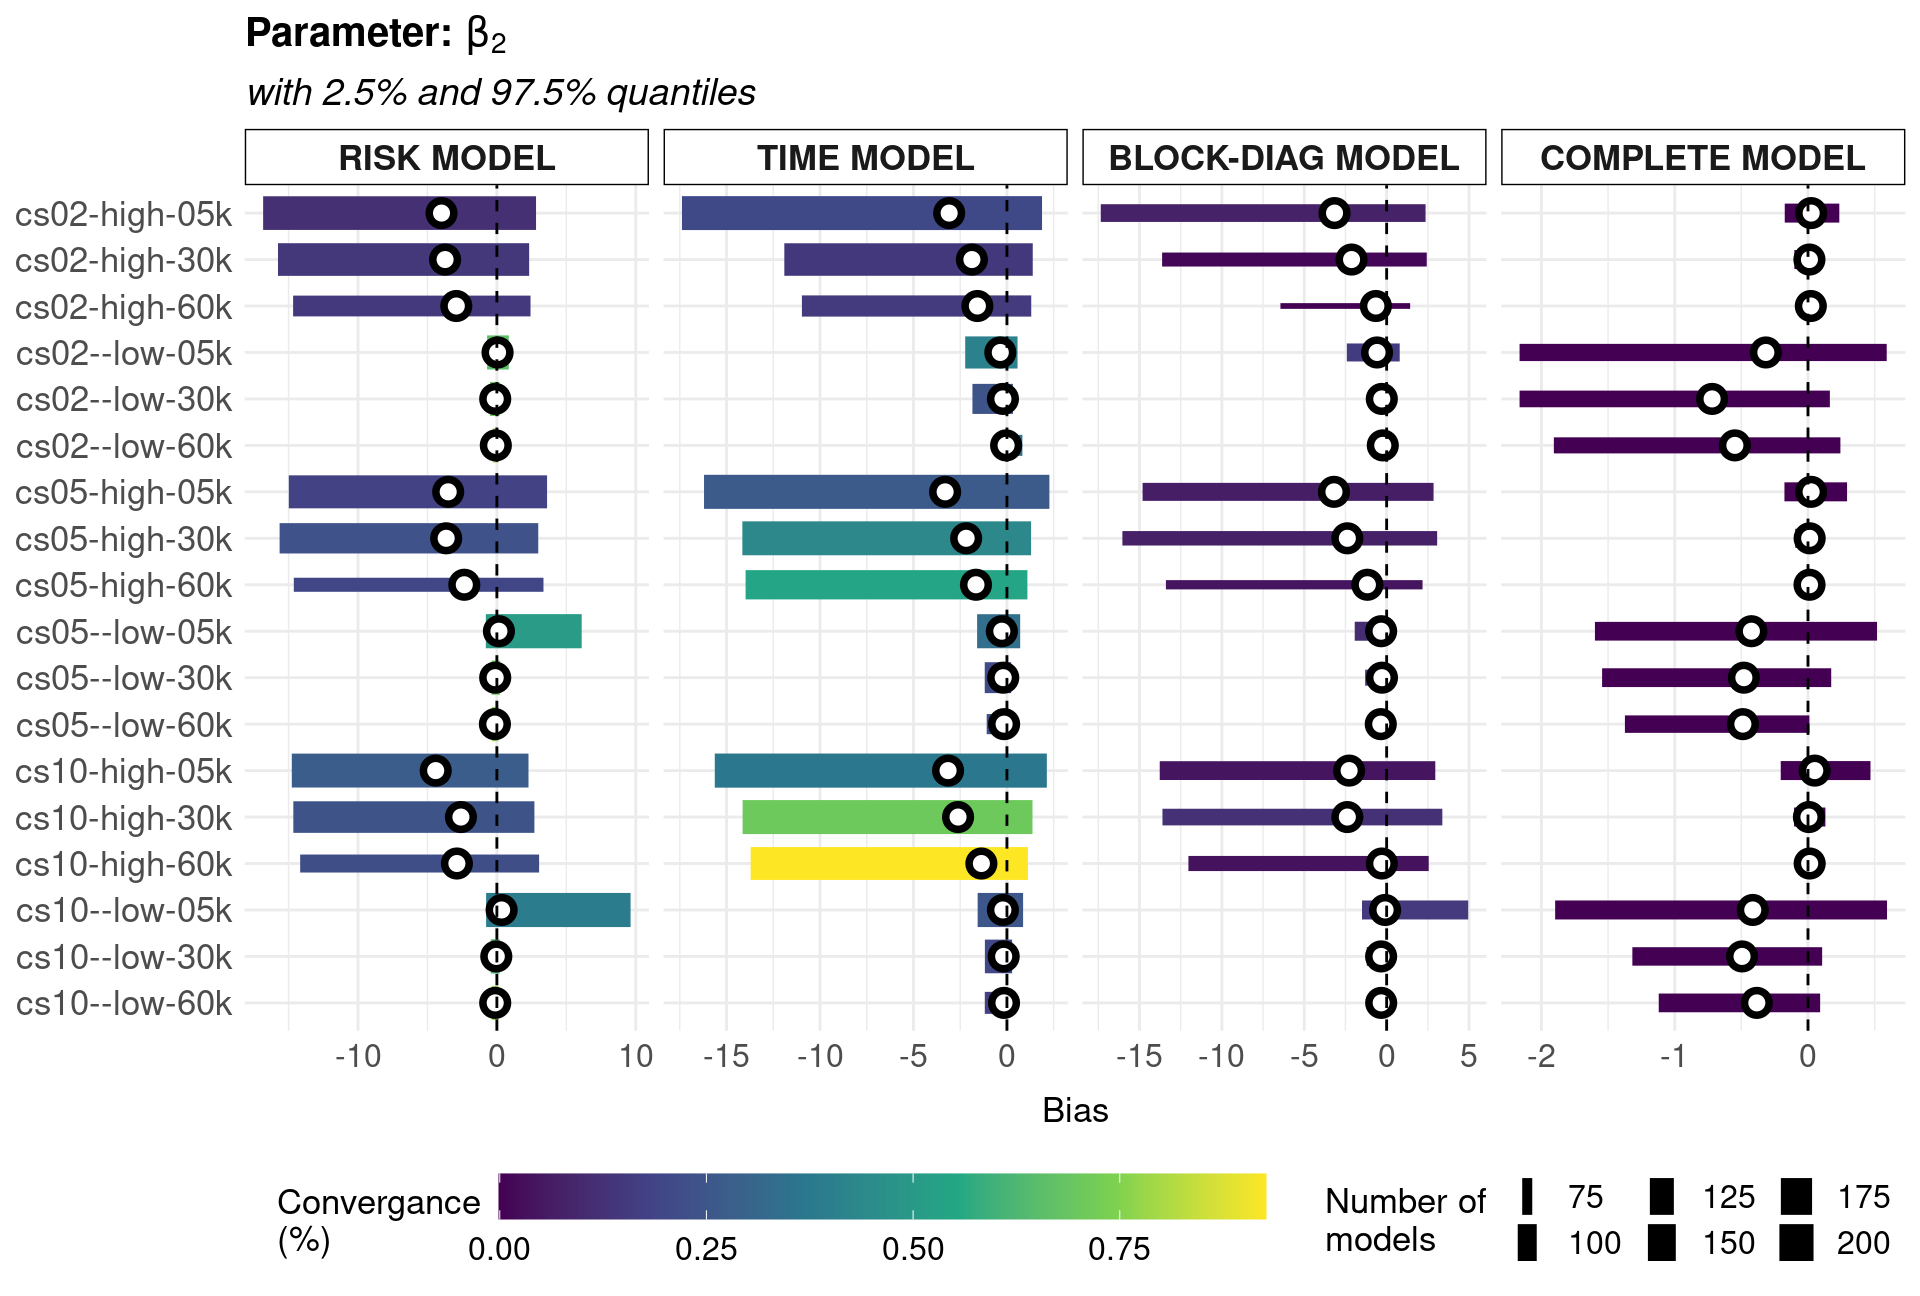
\includegraphics[width=\textwidth]{bias2plot-2.png}\\
 \begin{footnotesize}
  SOURCE: The author (2021).
 \end{footnotesize}
 \label{fig:biasbeta2}
\end{figure}

\begin{figure}[H]
 \setlength{\abovecaptionskip}{.0001pt}
 \caption{PARAMETER BIAS WITH 2.5\% AND 97.5\% QUANTILES}
 \vspace{0.2cm}\centering
 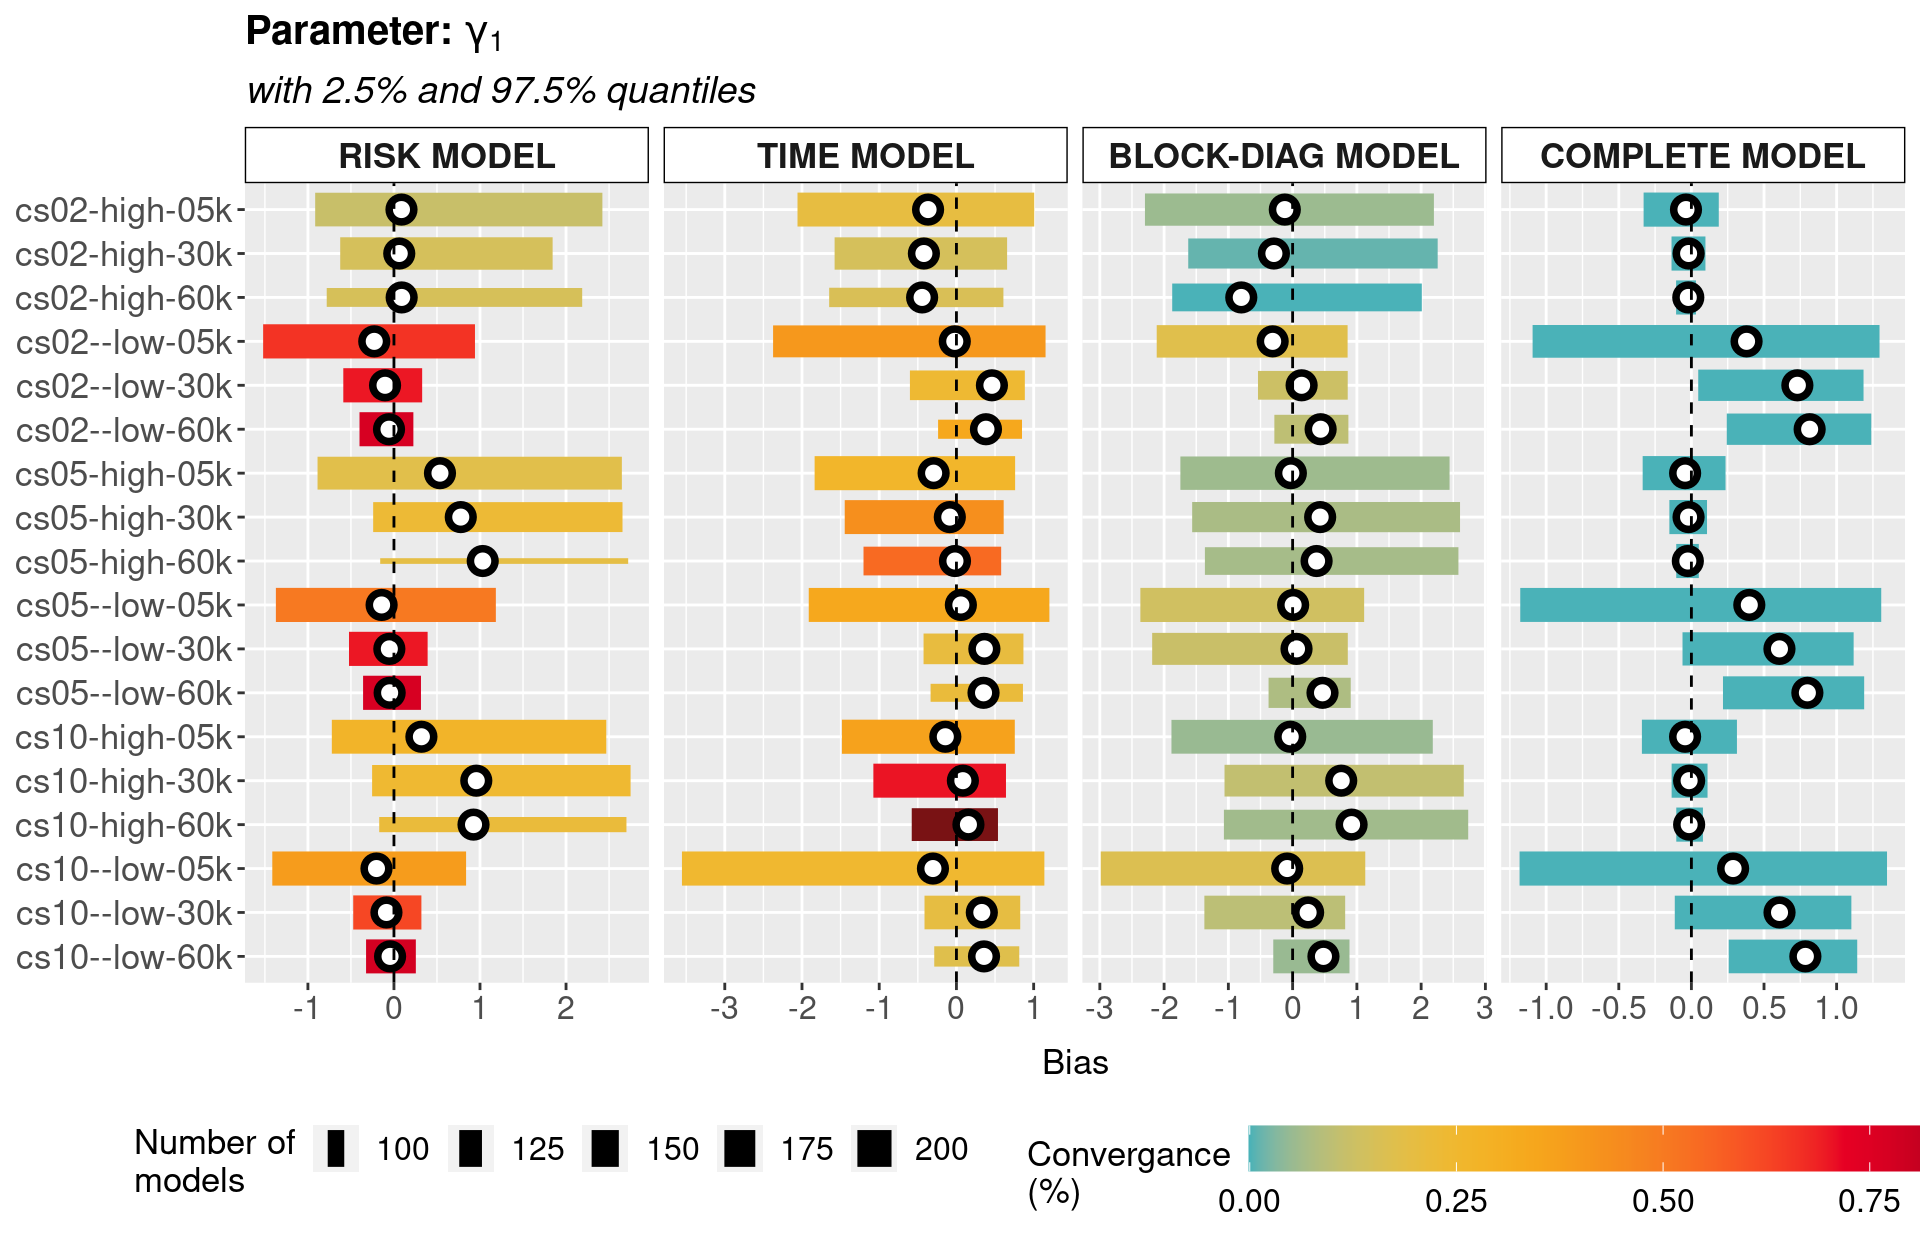
\includegraphics[width=\textwidth]{bias2plot-3.png}\\
 \begin{footnotesize}
  SOURCE: The author (2021).
 \end{footnotesize}
 \label{fig:biasgama1}
\end{figure}

\begin{figure}[H]
 \setlength{\abovecaptionskip}{.0001pt}
 \caption{PARAMETER BIAS WITH 2.5\% AND 97.5\% QUANTILES}
 \vspace{0.2cm}\centering
 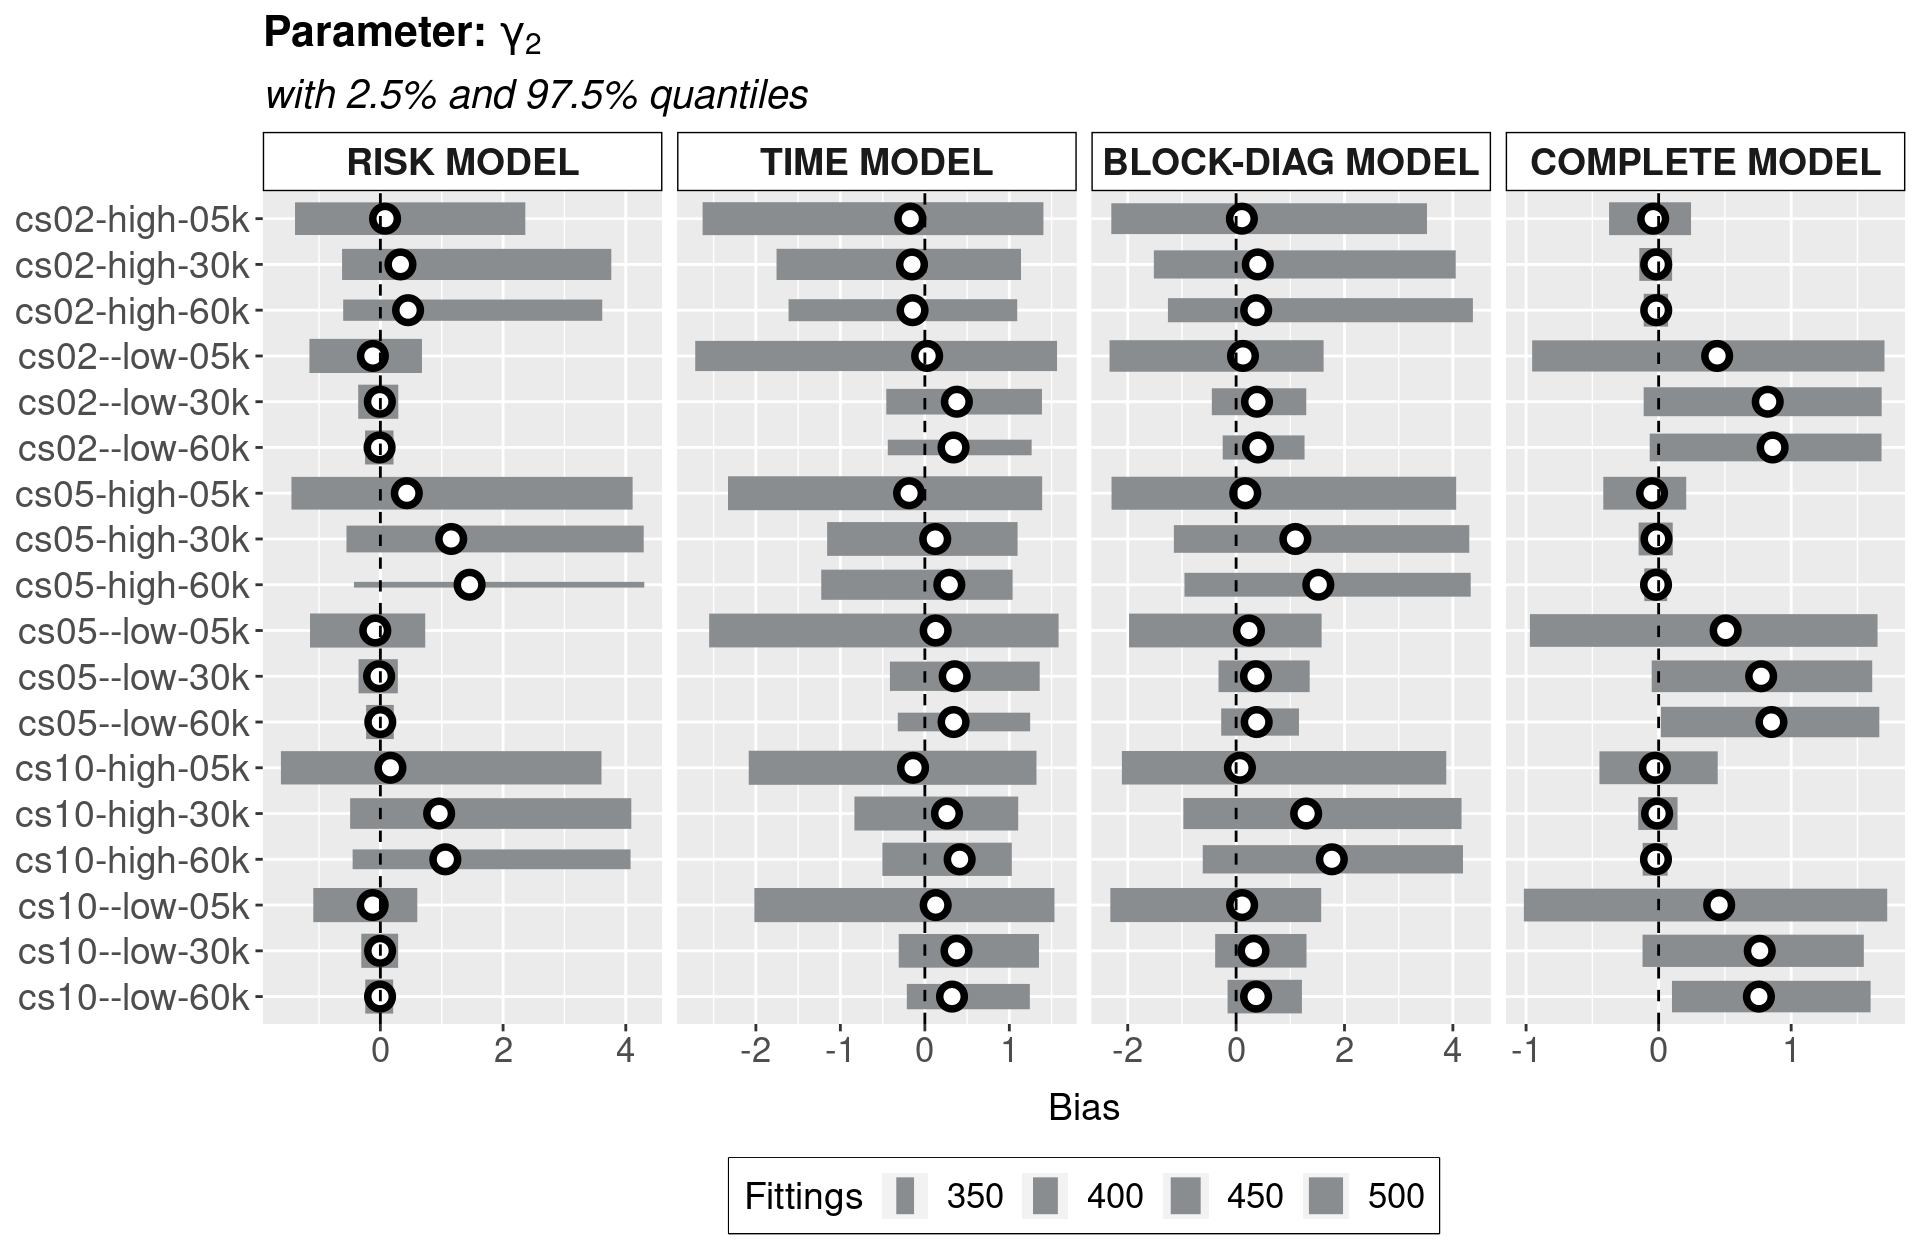
\includegraphics[width=\textwidth]{bias2plot-4.png}\\
 \begin{footnotesize}
  SOURCE: The author (2021).
 \end{footnotesize}
 \label{fig:biasgama2}
\end{figure}

\begin{figure}[H]
 \setlength{\abovecaptionskip}{.0001pt}
 \caption{PARAMETER BIAS WITH 2.5\% AND 97.5\% QUANTILES}
 \vspace{0.2cm}\centering
 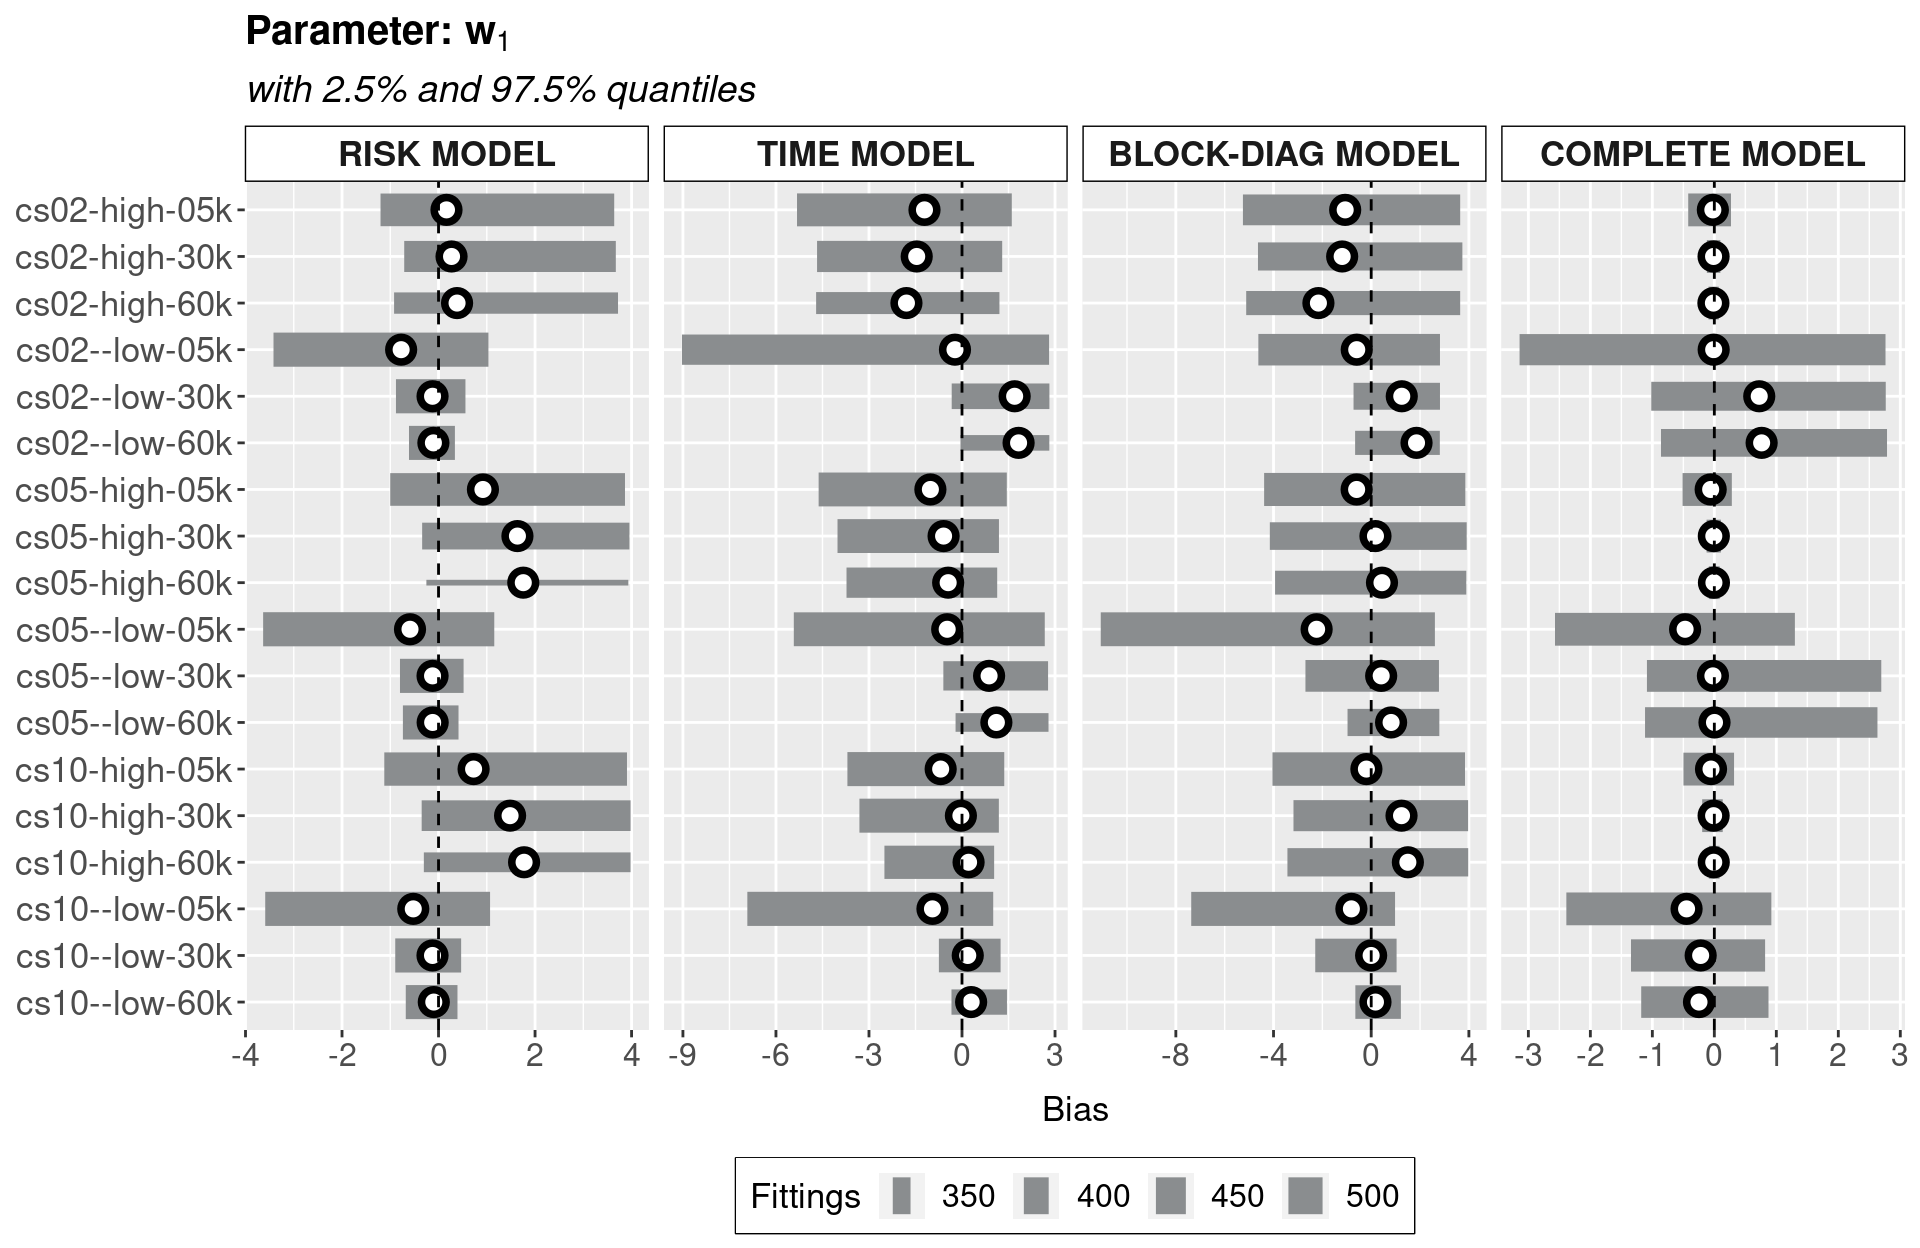
\includegraphics[width=\textwidth]{bias2plot-5.png}\\
 \begin{footnotesize}
  SOURCE: The author (2021).
 \end{footnotesize}
 \label{fig:biasw1}
\end{figure}

\begin{figure}[H]
 \setlength{\abovecaptionskip}{.0001pt}
 \caption{PARAMETER BIAS WITH 2.5\% AND 97.5\% QUANTILES}
 \vspace{0.2cm}\centering
 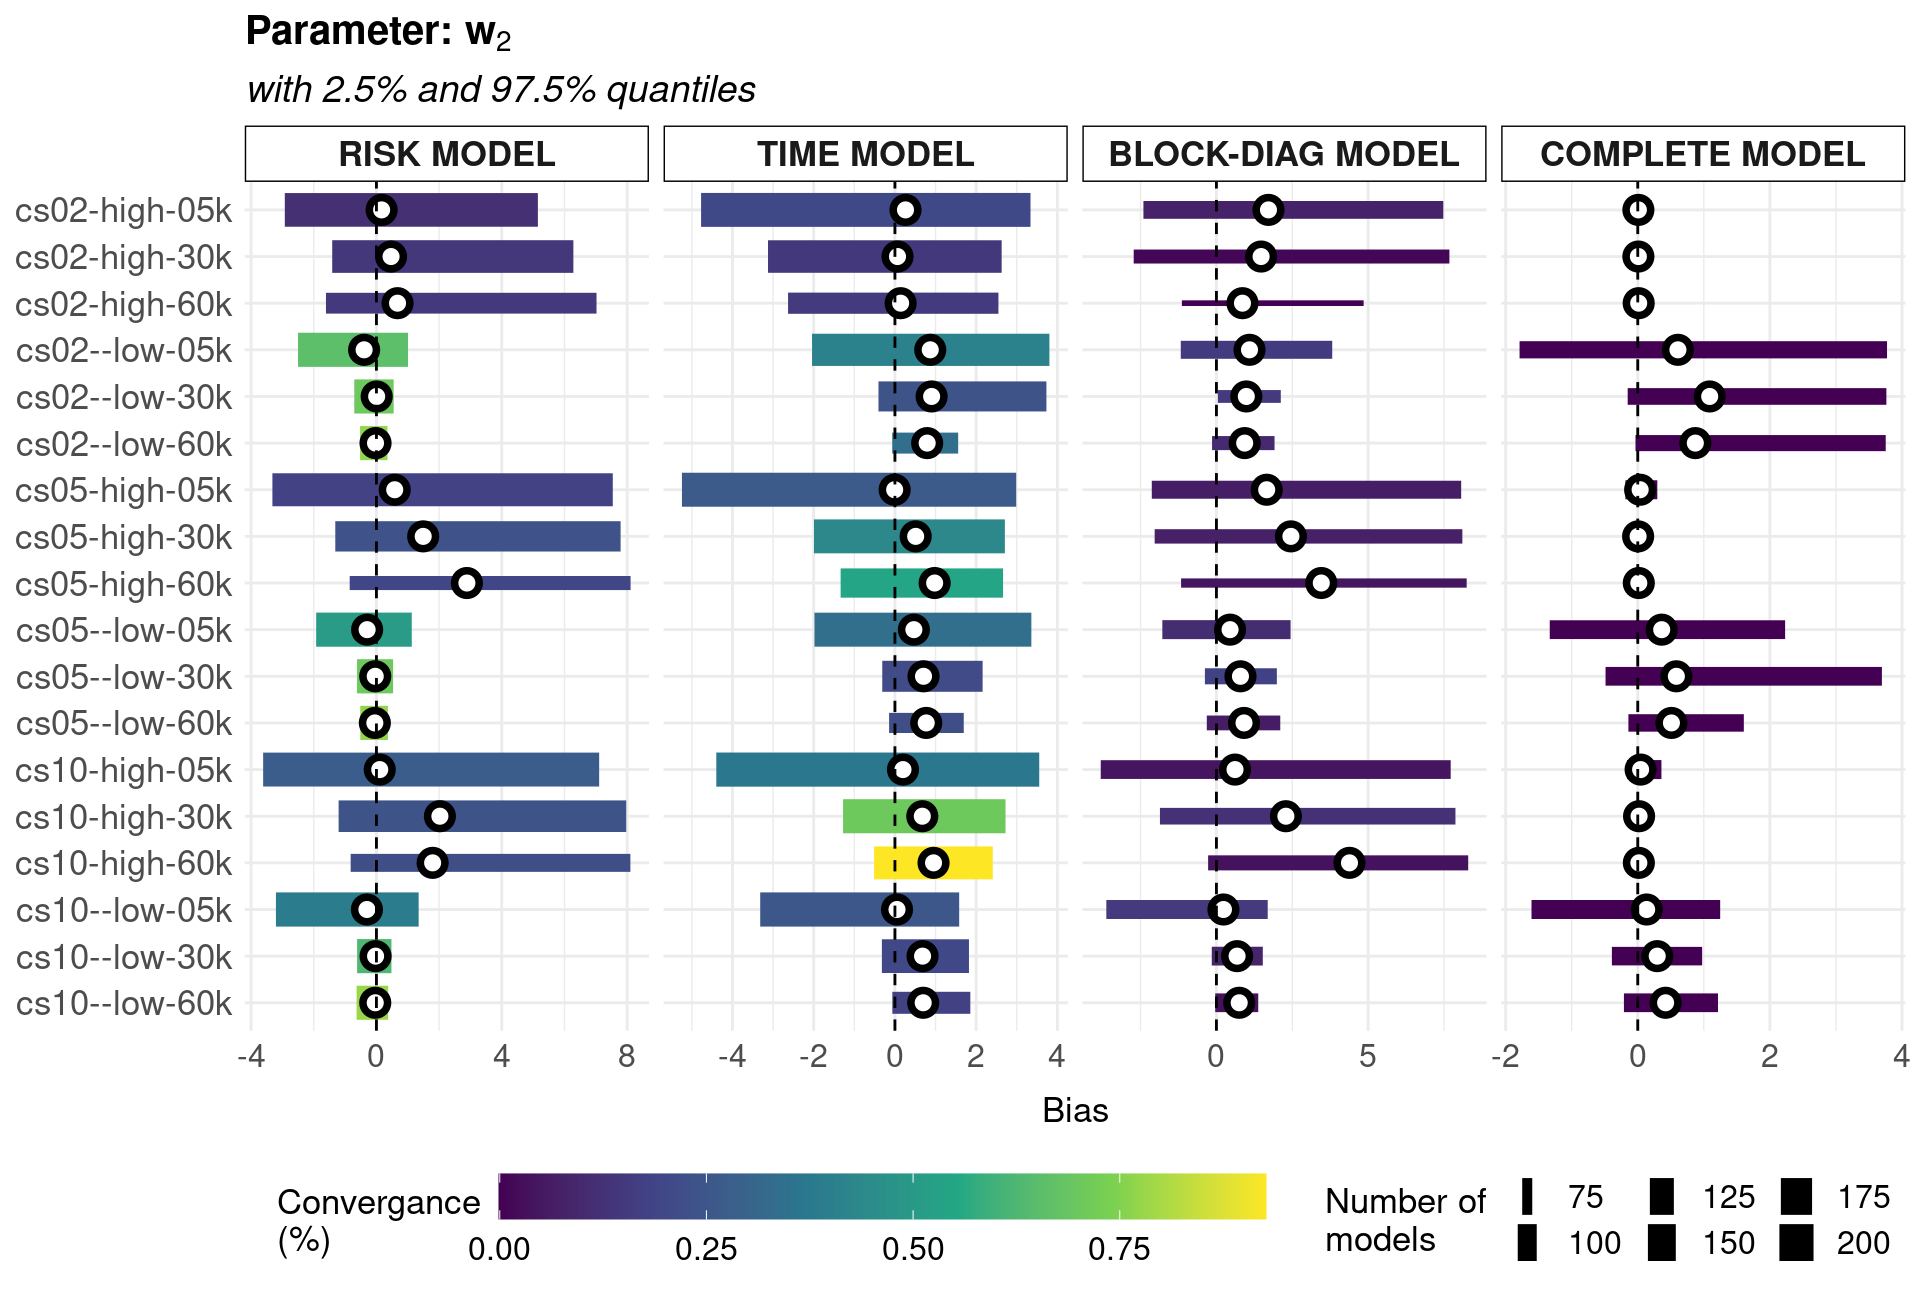
\includegraphics[width=\textwidth]{bias2plot-6.png}\\
 \begin{footnotesize}
  SOURCE: The author (2021).
 \end{footnotesize}
 \label{fig:biasw2}
\end{figure}

\begin{figure}[H]
 \setlength{\abovecaptionskip}{.0001pt}
 \caption{PARAMETER BIAS WITH 2.5\% AND 97.5\% QUANTILES}
 \vspace{0.2cm}\centering
 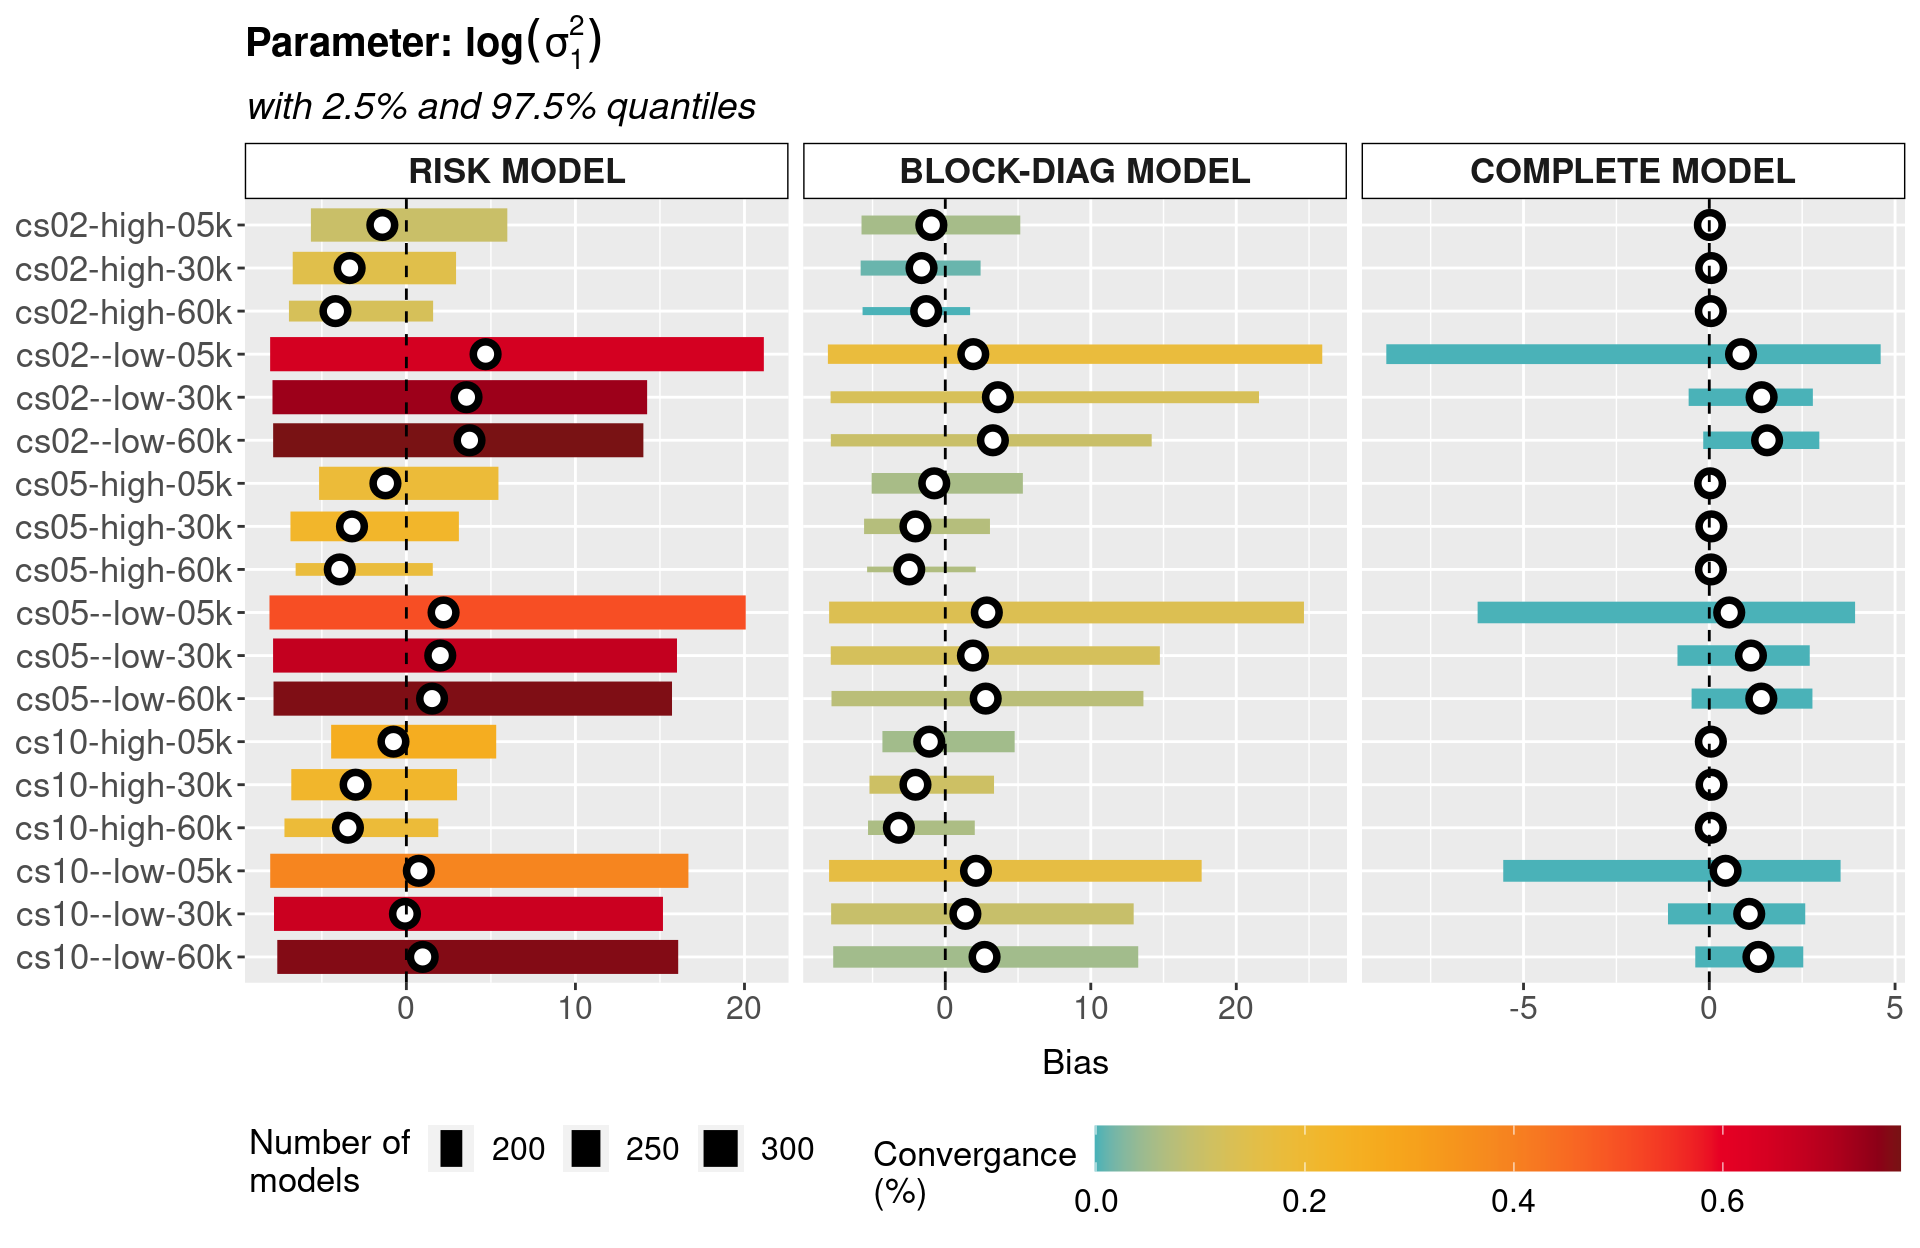
\includegraphics[width=\textwidth]{bias2plot-7.png}\\
 \begin{footnotesize}
  SOURCE: The author (2021).
 \end{footnotesize}
 \label{fig:biaslogs2_1}
\end{figure}

\begin{figure}[H]
 \setlength{\abovecaptionskip}{.0001pt}
 \caption{PARAMETER BIAS WITH 2.5\% AND 97.5\% QUANTILES}
 \vspace{0.2cm}\centering
 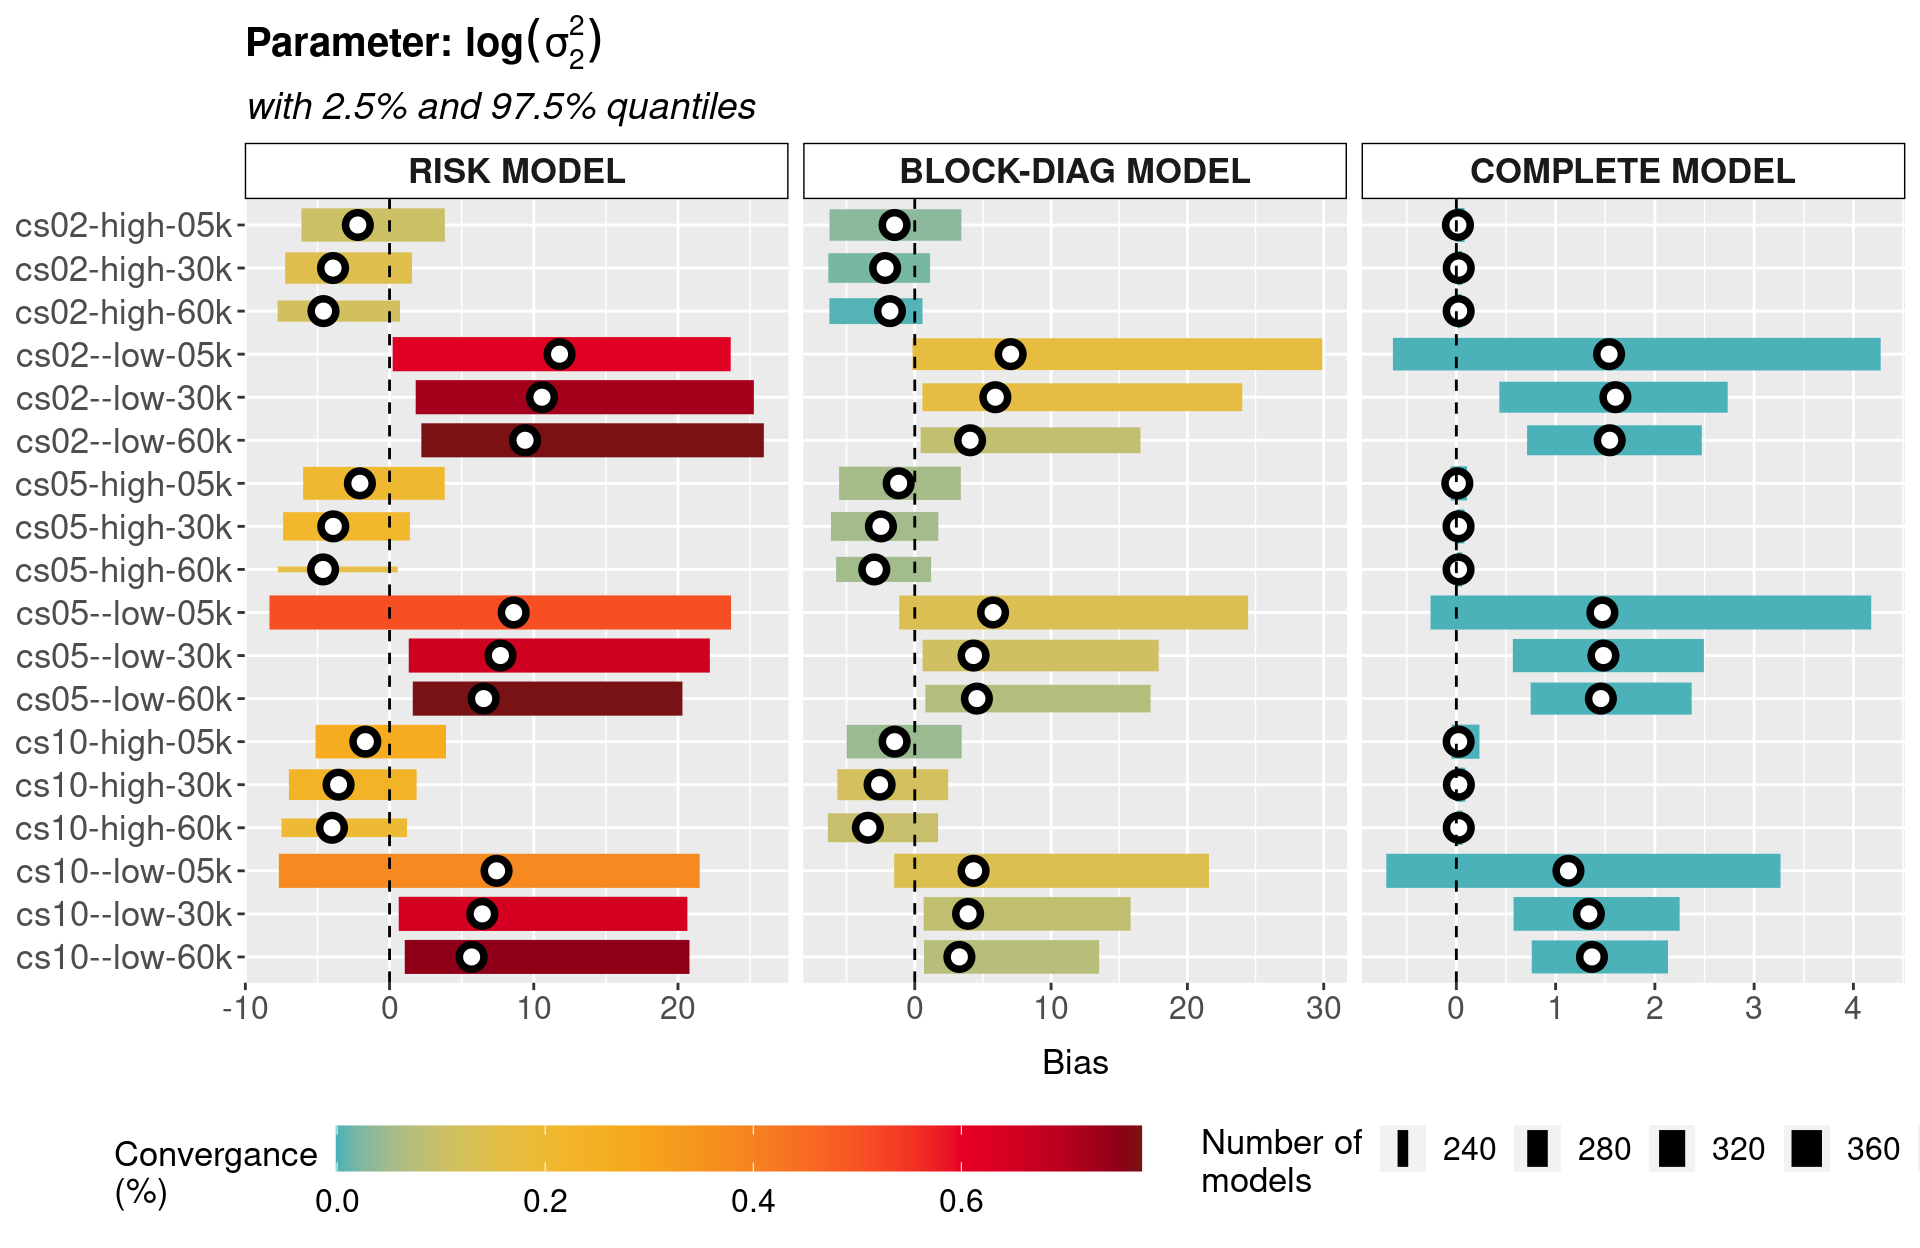
\includegraphics[width=\textwidth]{bias2plot-8.png}\\
 \begin{footnotesize}
  SOURCE: The author (2021).
 \end{footnotesize}
 \label{fig:biaslogs2_2}
\end{figure}

\begin{figure}[H]
 \setlength{\abovecaptionskip}{.0001pt}
 \caption{PARAMETER BIAS WITH 2.5\% AND 97.5\% QUANTILES}
 \vspace{0.2cm}\centering
 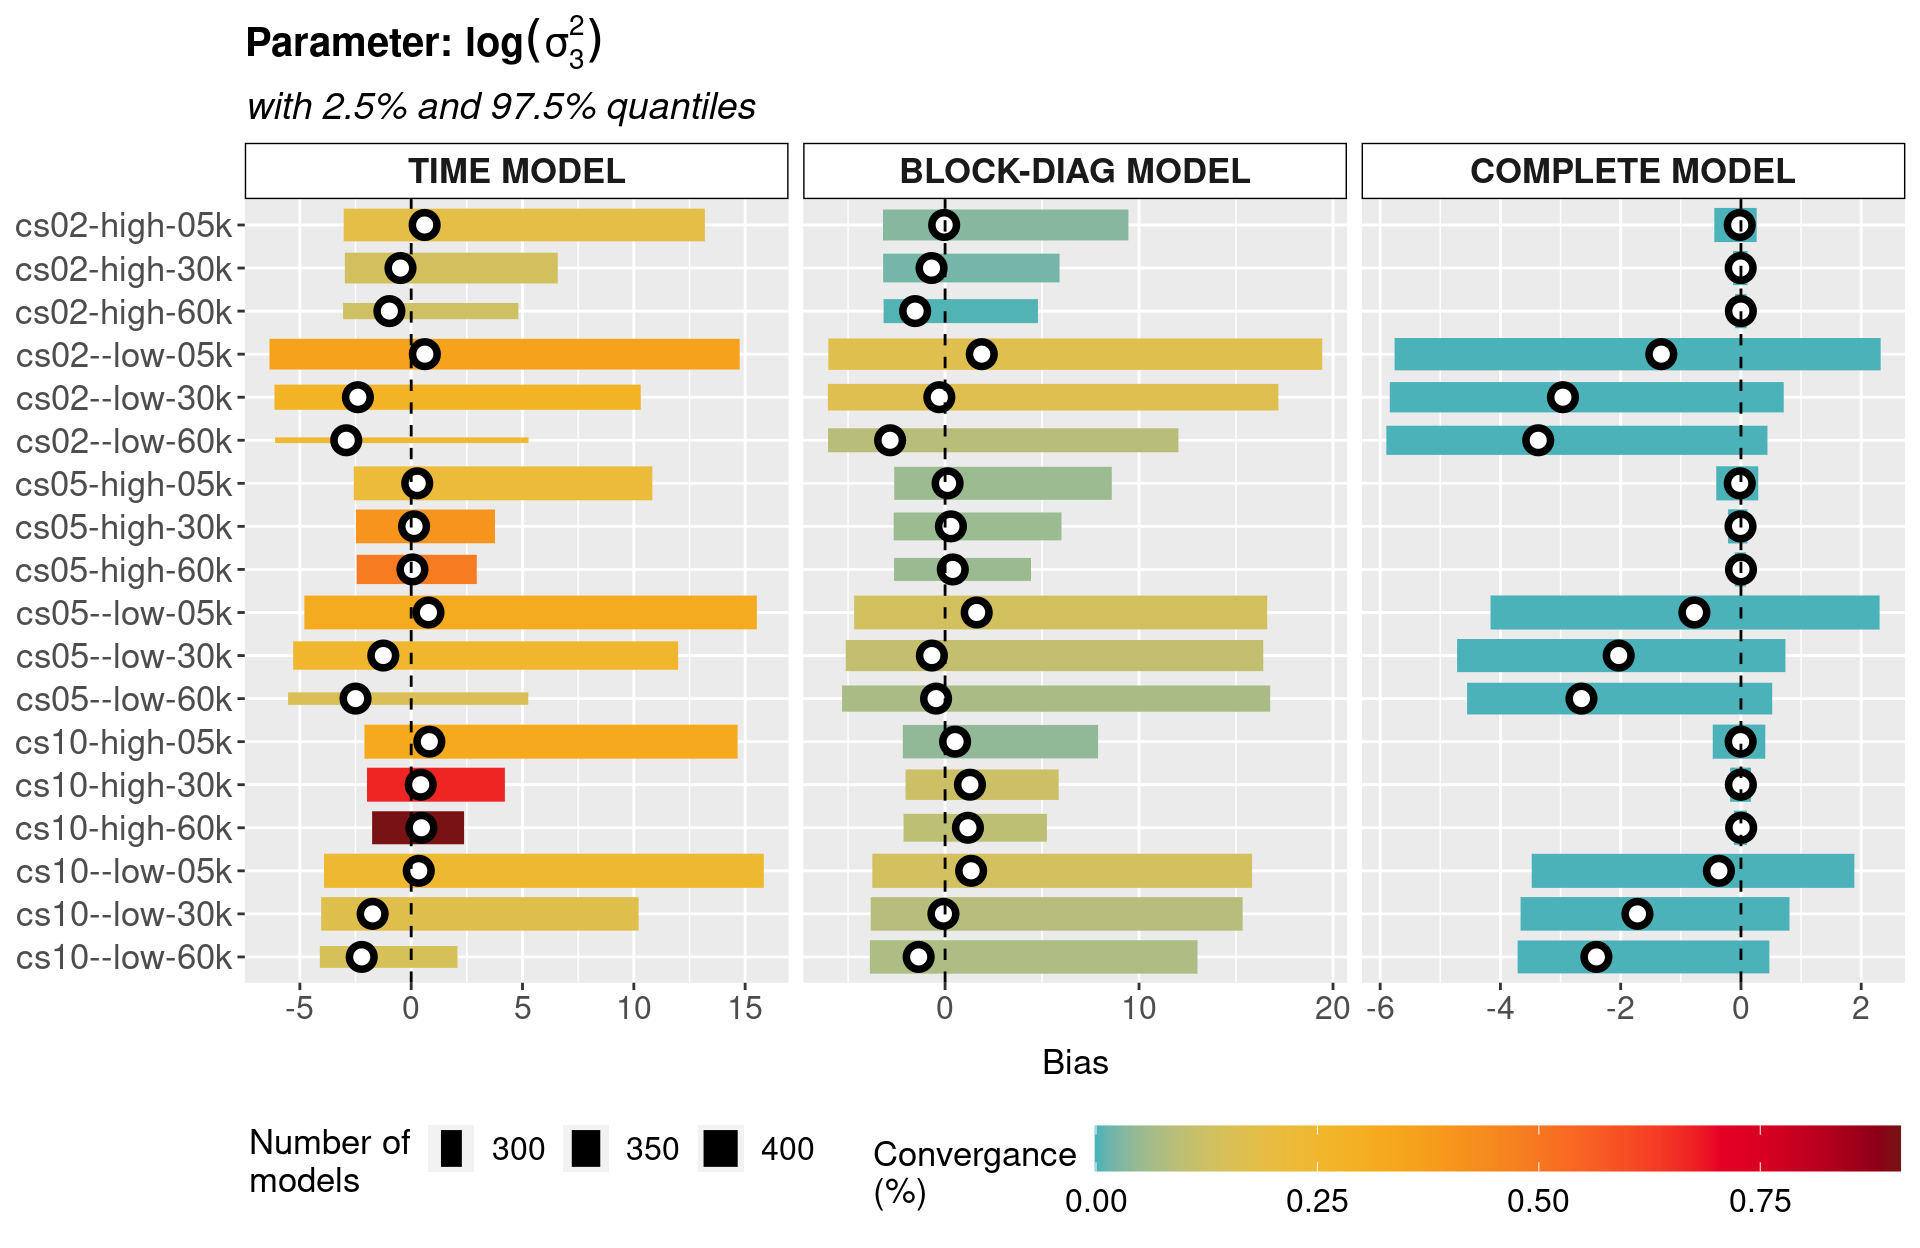
\includegraphics[width=\textwidth]{bias2plot-9.png}\\
 \begin{footnotesize}
  SOURCE: The author (2021).
 \end{footnotesize}
 \label{fig:biaslogs2_3}
\end{figure}

\begin{figure}[H]
 \setlength{\abovecaptionskip}{.0001pt}
 \caption{PARAMETER BIAS WITH 2.5\% AND 97.5\% QUANTILES}
 \vspace{0.2cm}\centering
 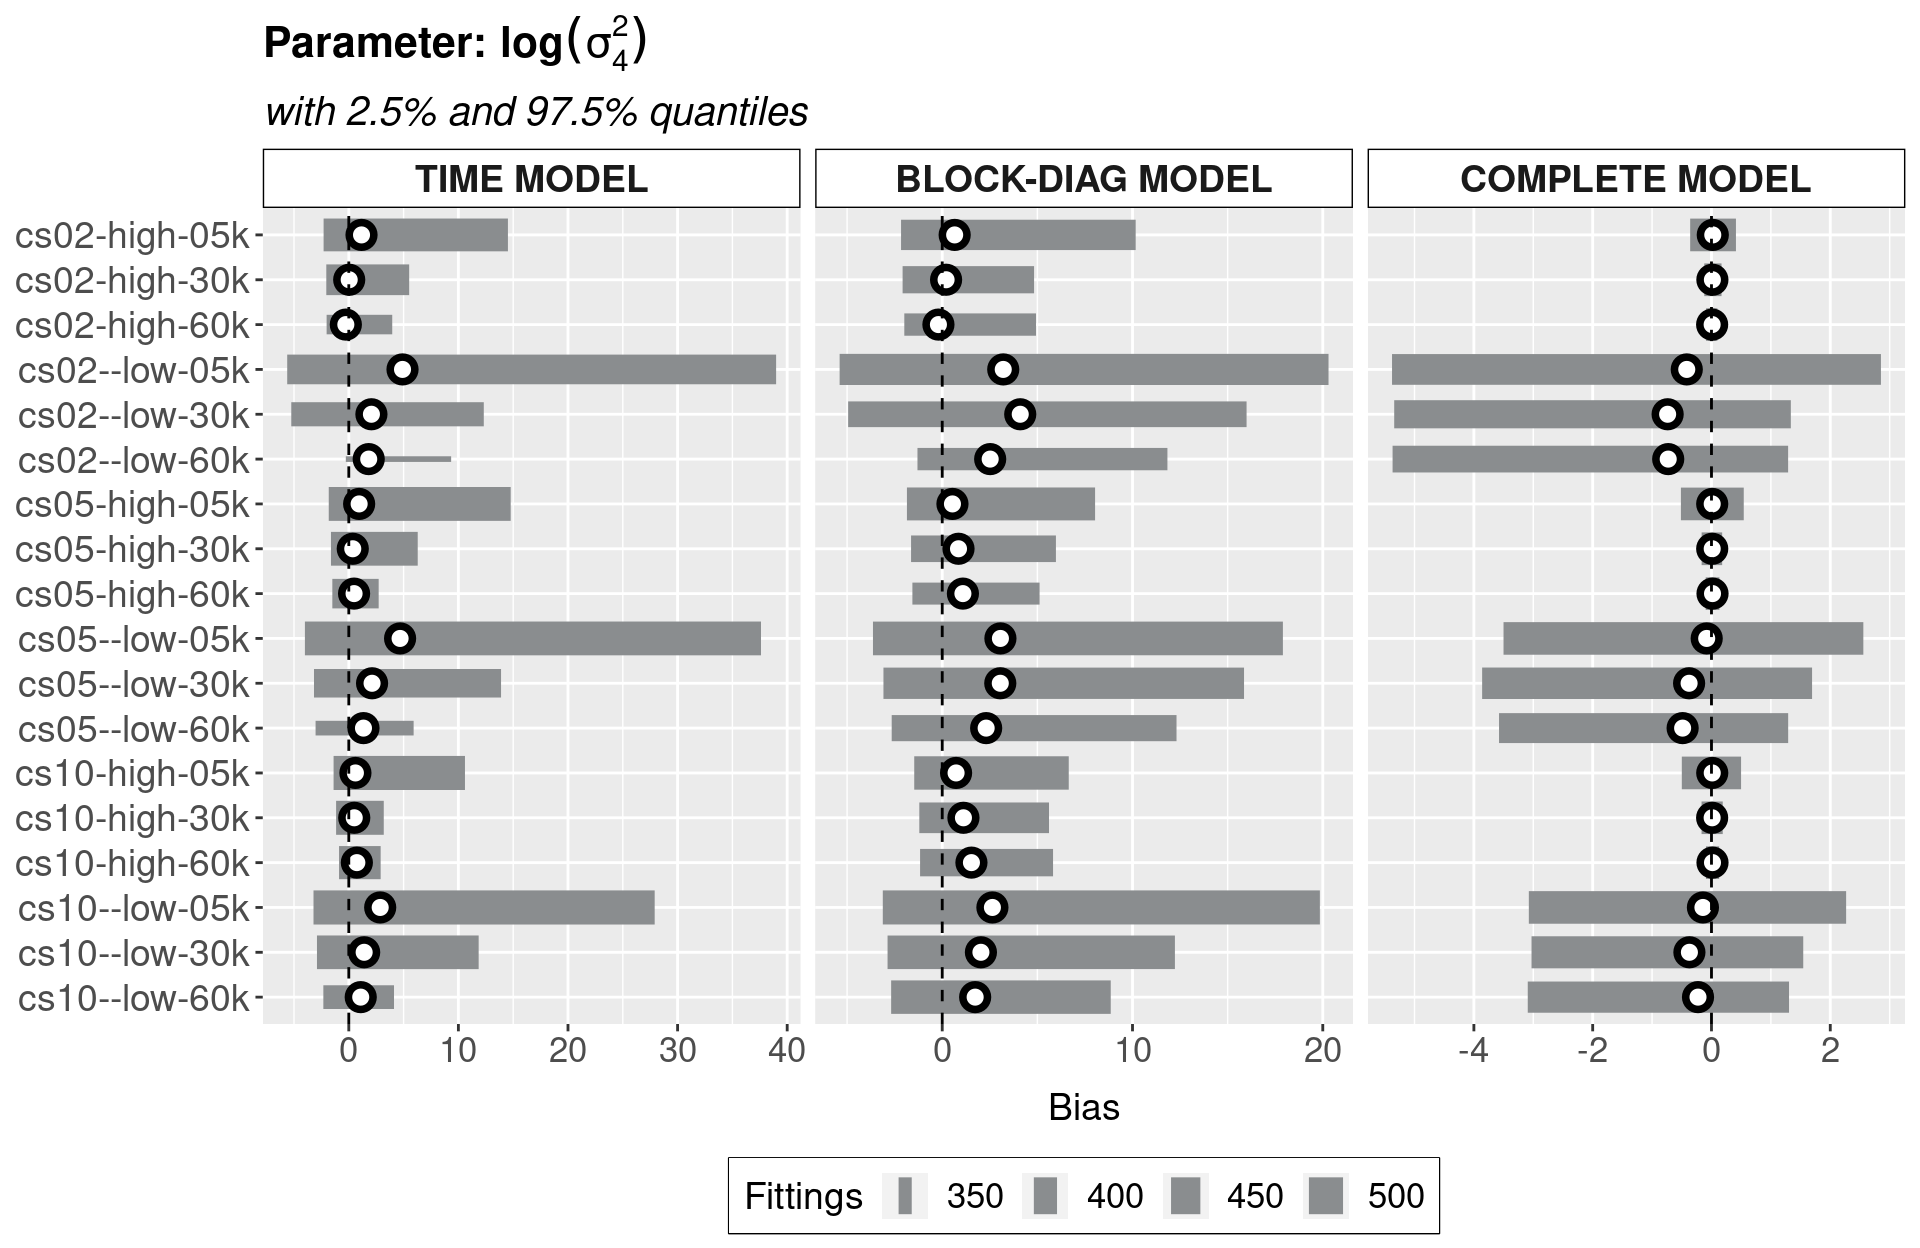
\includegraphics[width=\textwidth]{bias2plot-10.png}\\
 \begin{footnotesize}
  SOURCE: The author (2021).
 \end{footnotesize}
 \label{fig:biaslogs2_4}
\end{figure}

%% \begin{figure}[H]
%%  \setlength{\abovecaptionskip}{.0001pt}
%%  \caption{BUILDING \(\Sigma\)}
%%  \vspace{0.2cm}\centering
%%  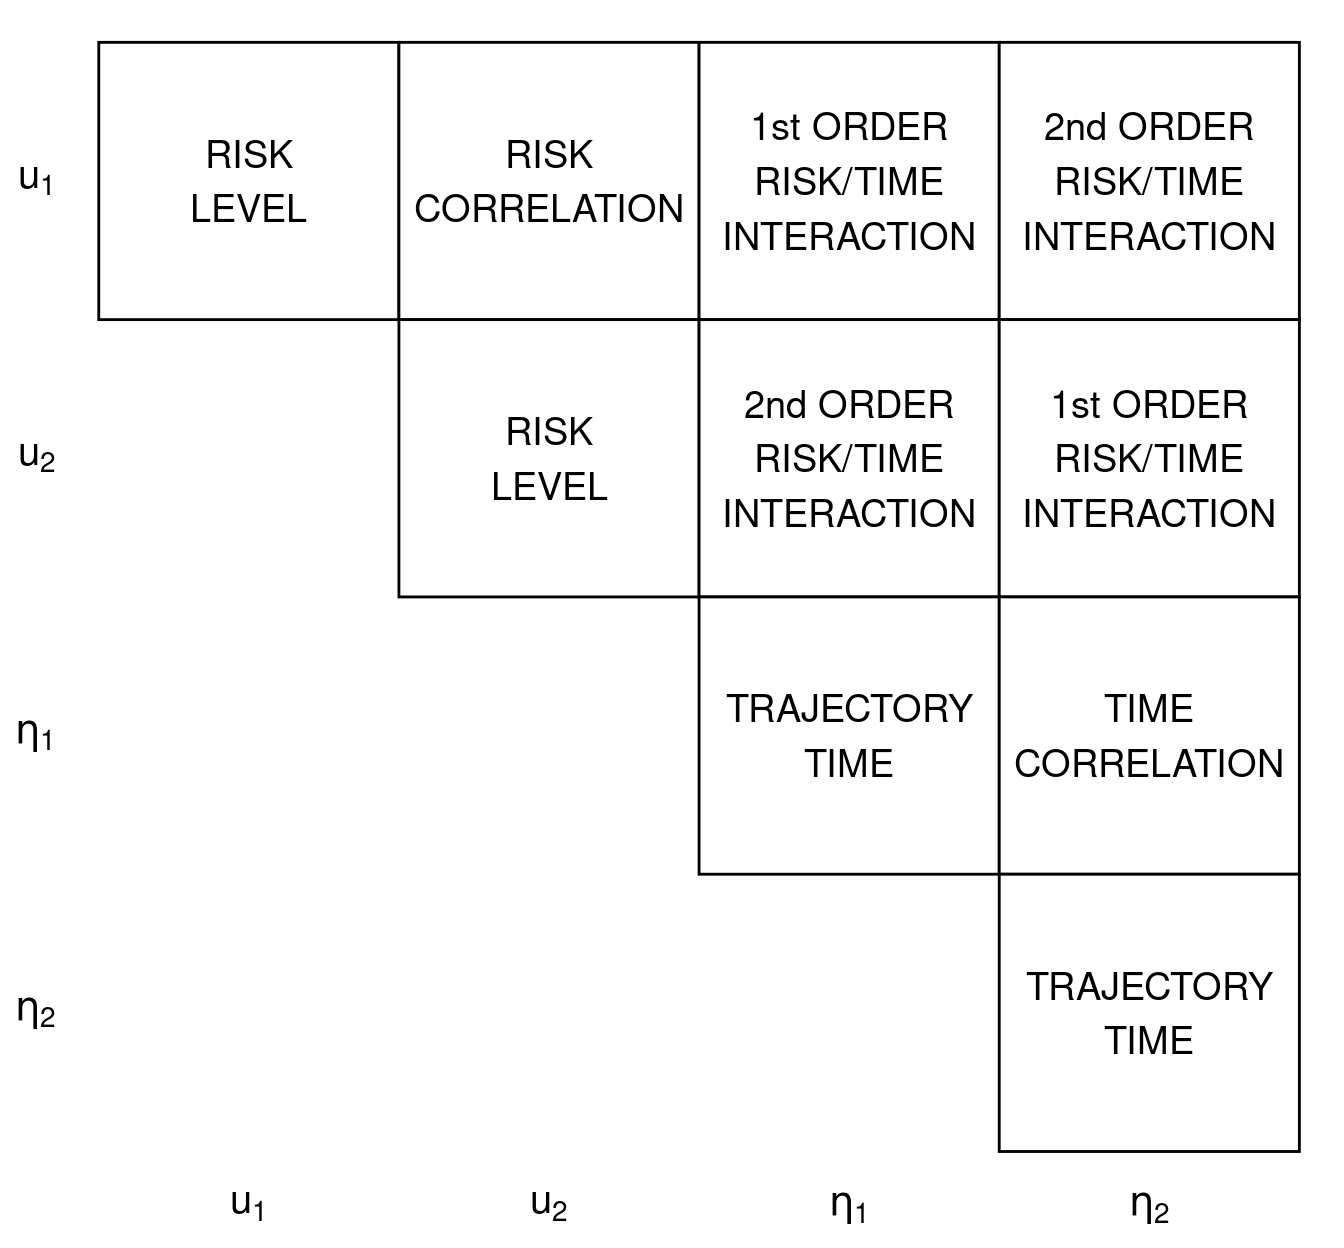
\includegraphics[width=0.75\textwidth]{buildingSigma-1.png}\\
%%  \begin{footnotesize}
%%   SOURCE: The author (2021).
%%  \end{footnotesize}
%%  \label{fig:buildingSigma}
%% \end{figure}

%% \begin{figure}[H]
%%  \setlength{\abovecaptionskip}{.0001pt}
%%  \caption{PARAMETERS CORRELATION}
%%  \vspace{0.2cm}\centering
%%  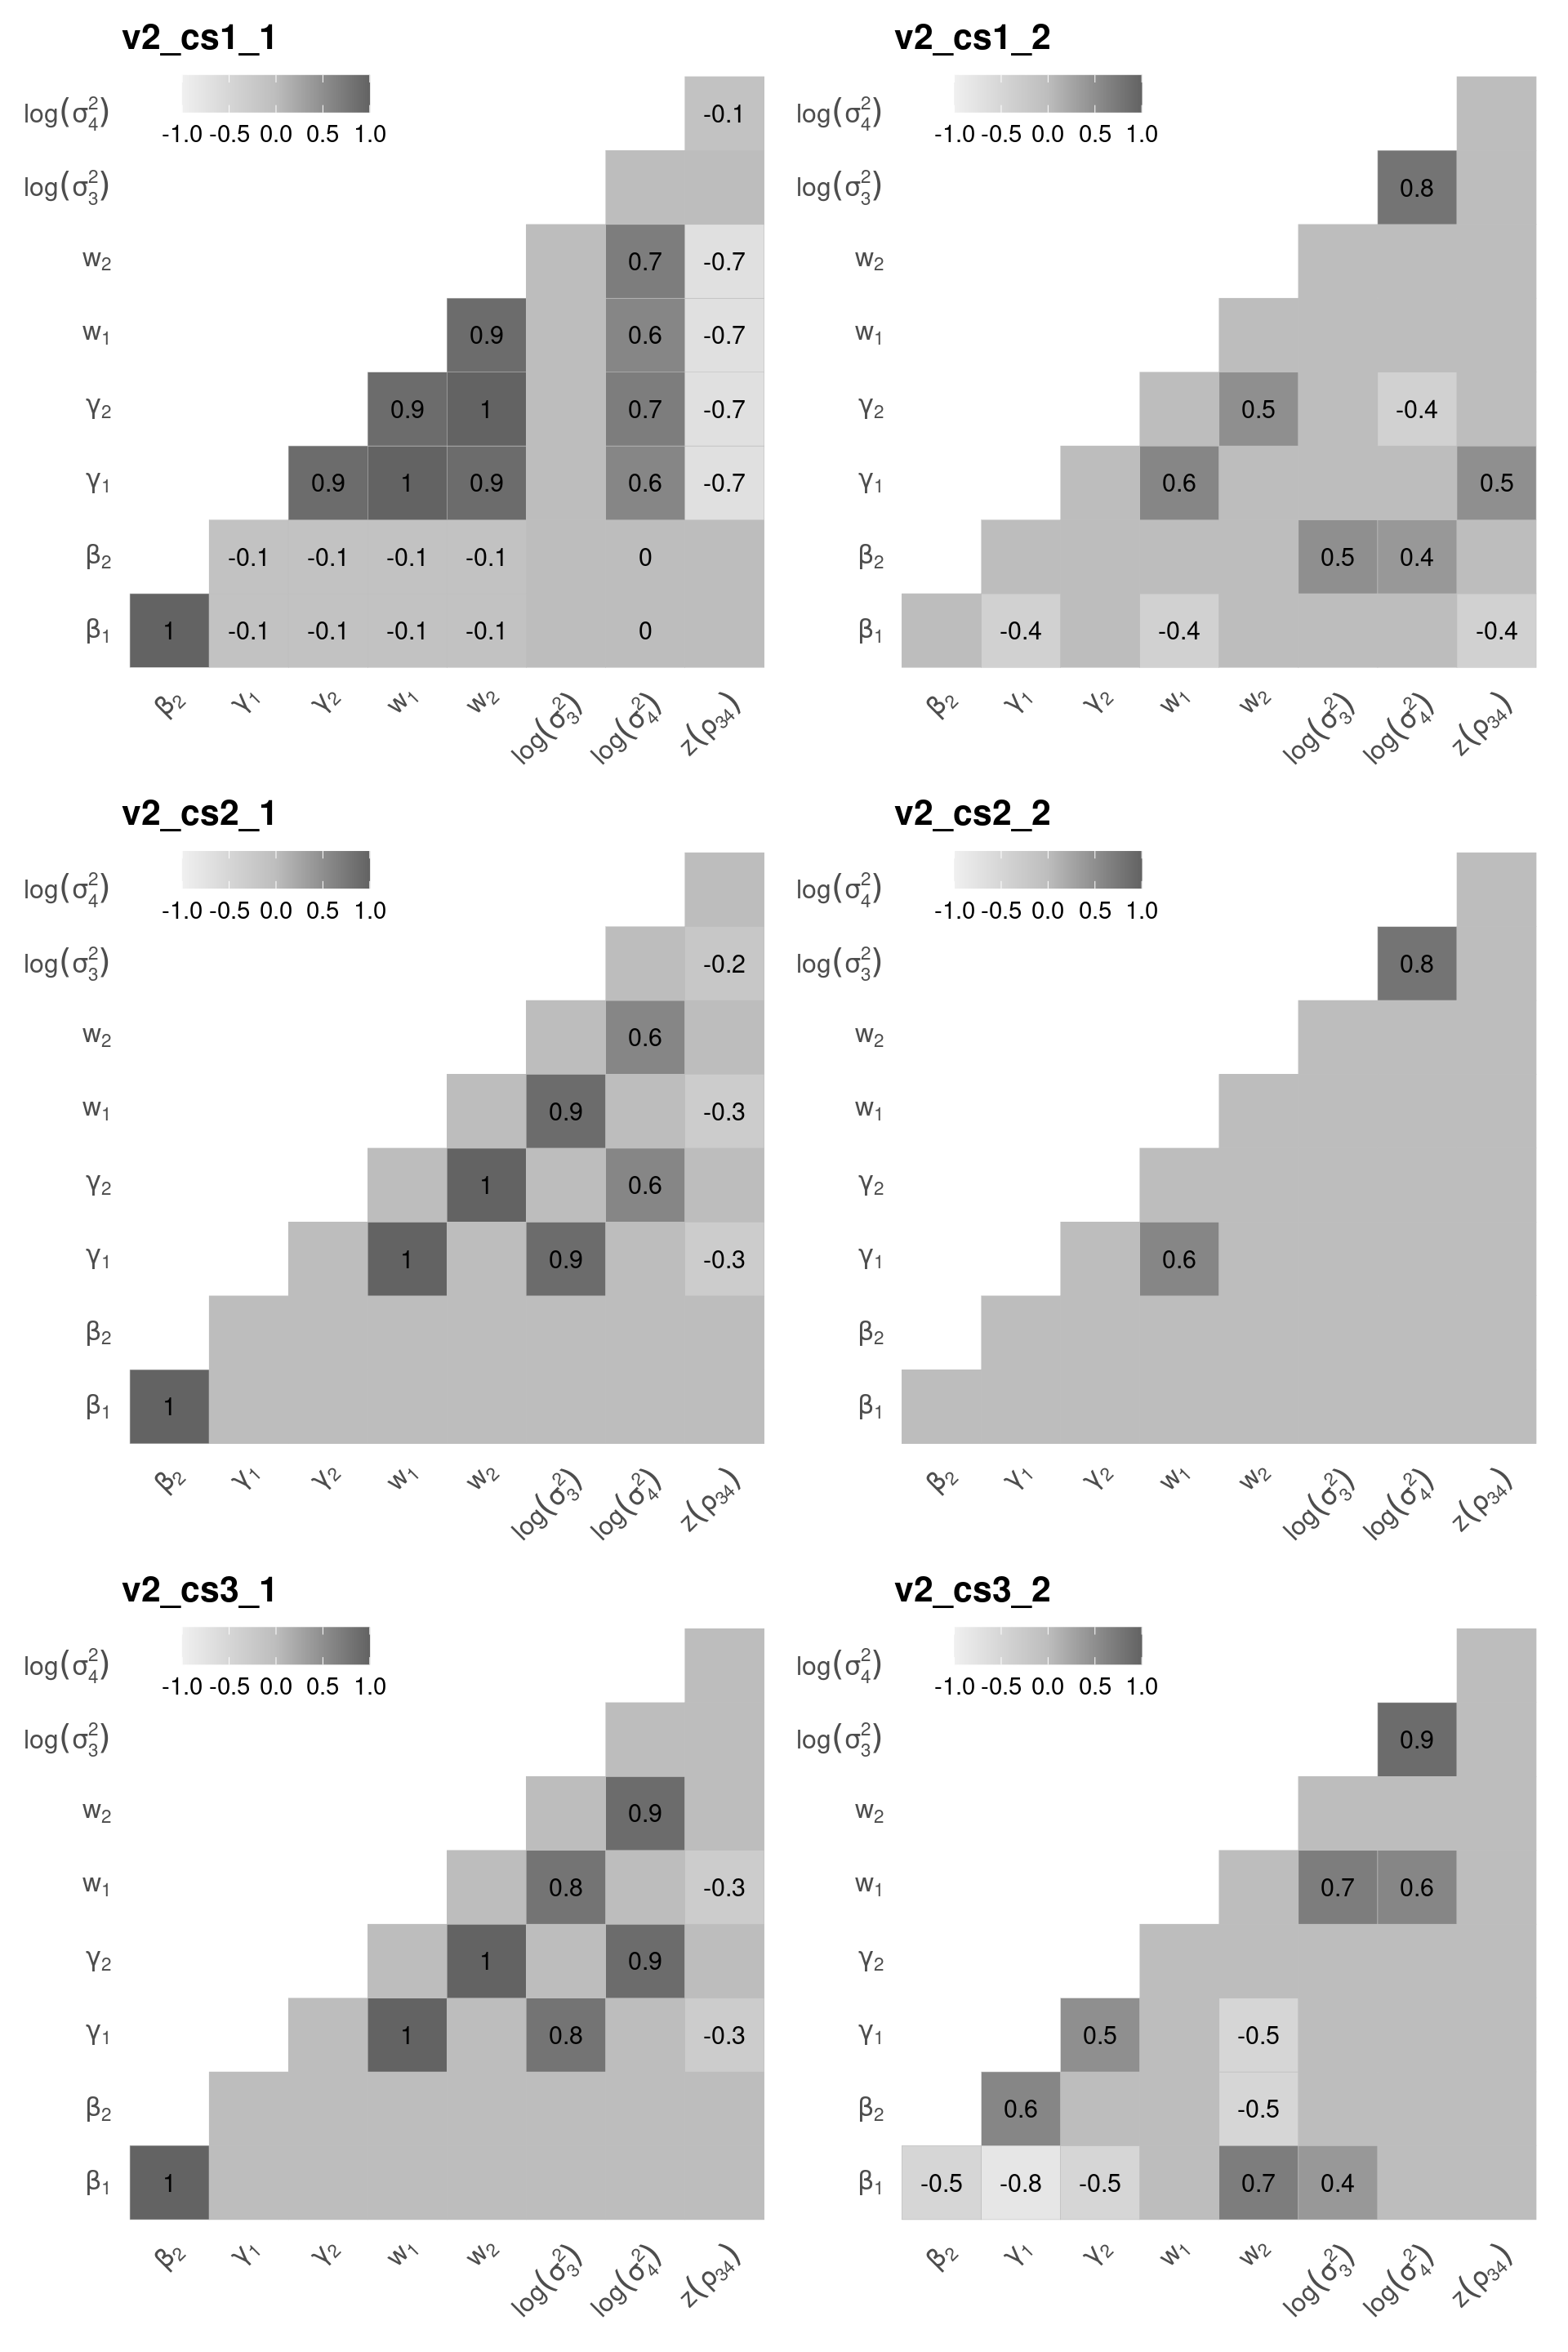
\includegraphics[width=\textwidth]{cor2plot-1.png}\\
%%  \begin{footnotesize}
%%   SOURCE: The author (2021).
%%  \end{footnotesize}
%%  \label{fig:cor2plot}
%% \end{figure}

%% \begin{figure}[H]
%%  \setlength{\abovecaptionskip}{.0001pt}
%%  \caption{VARIANCE-COVARIANCE MATRIX UPPER-TRIANGULAR COMPONENTS}
%%  \vspace{0.2cm}\centering
%%  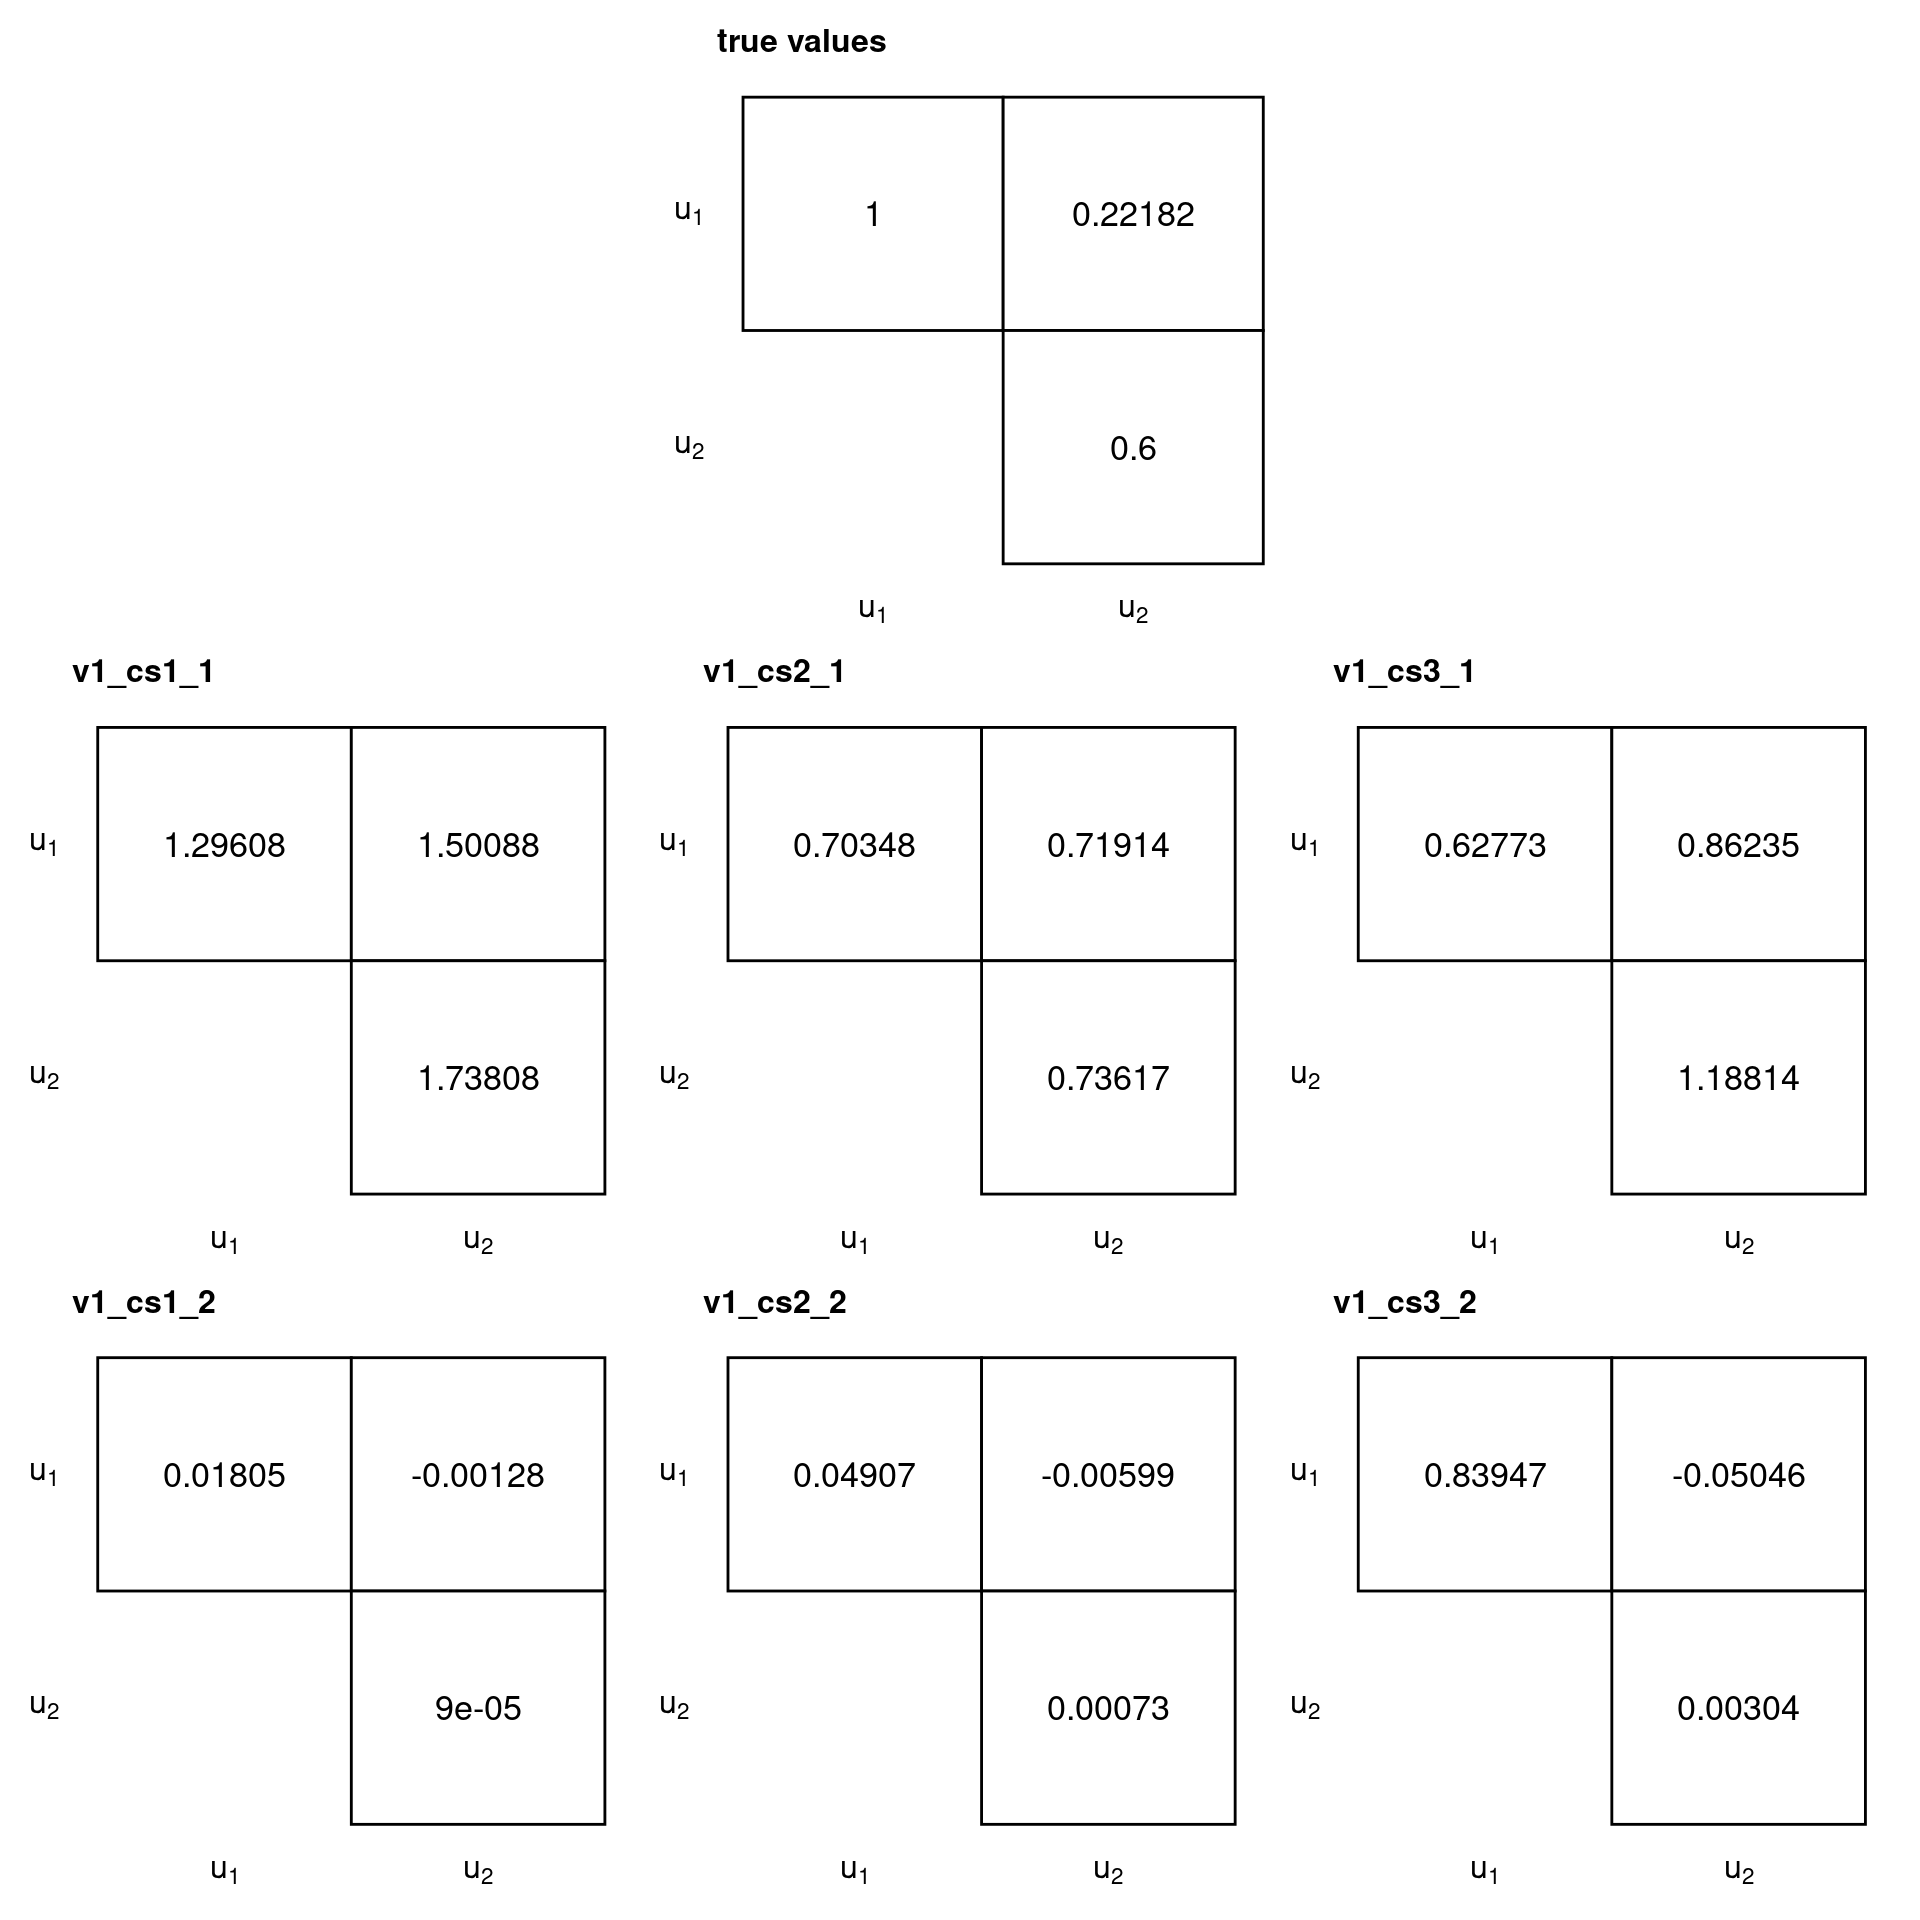
\includegraphics[width=\textwidth]{vcovs-1.png}\\
%%  \begin{footnotesize}
%%   SOURCE: The author (2021).
%%  \end{footnotesize}
%%  \label{fig:vcovs}
%% \end{figure}

%% \begin{figure}[H]
%%  \setlength{\abovecaptionskip}{.0001pt}
%%  \caption{CUMULATIVE INCIDENCE FUNCTIONS (CIFs)}
%%  \vspace{0.2cm}\centering
%%  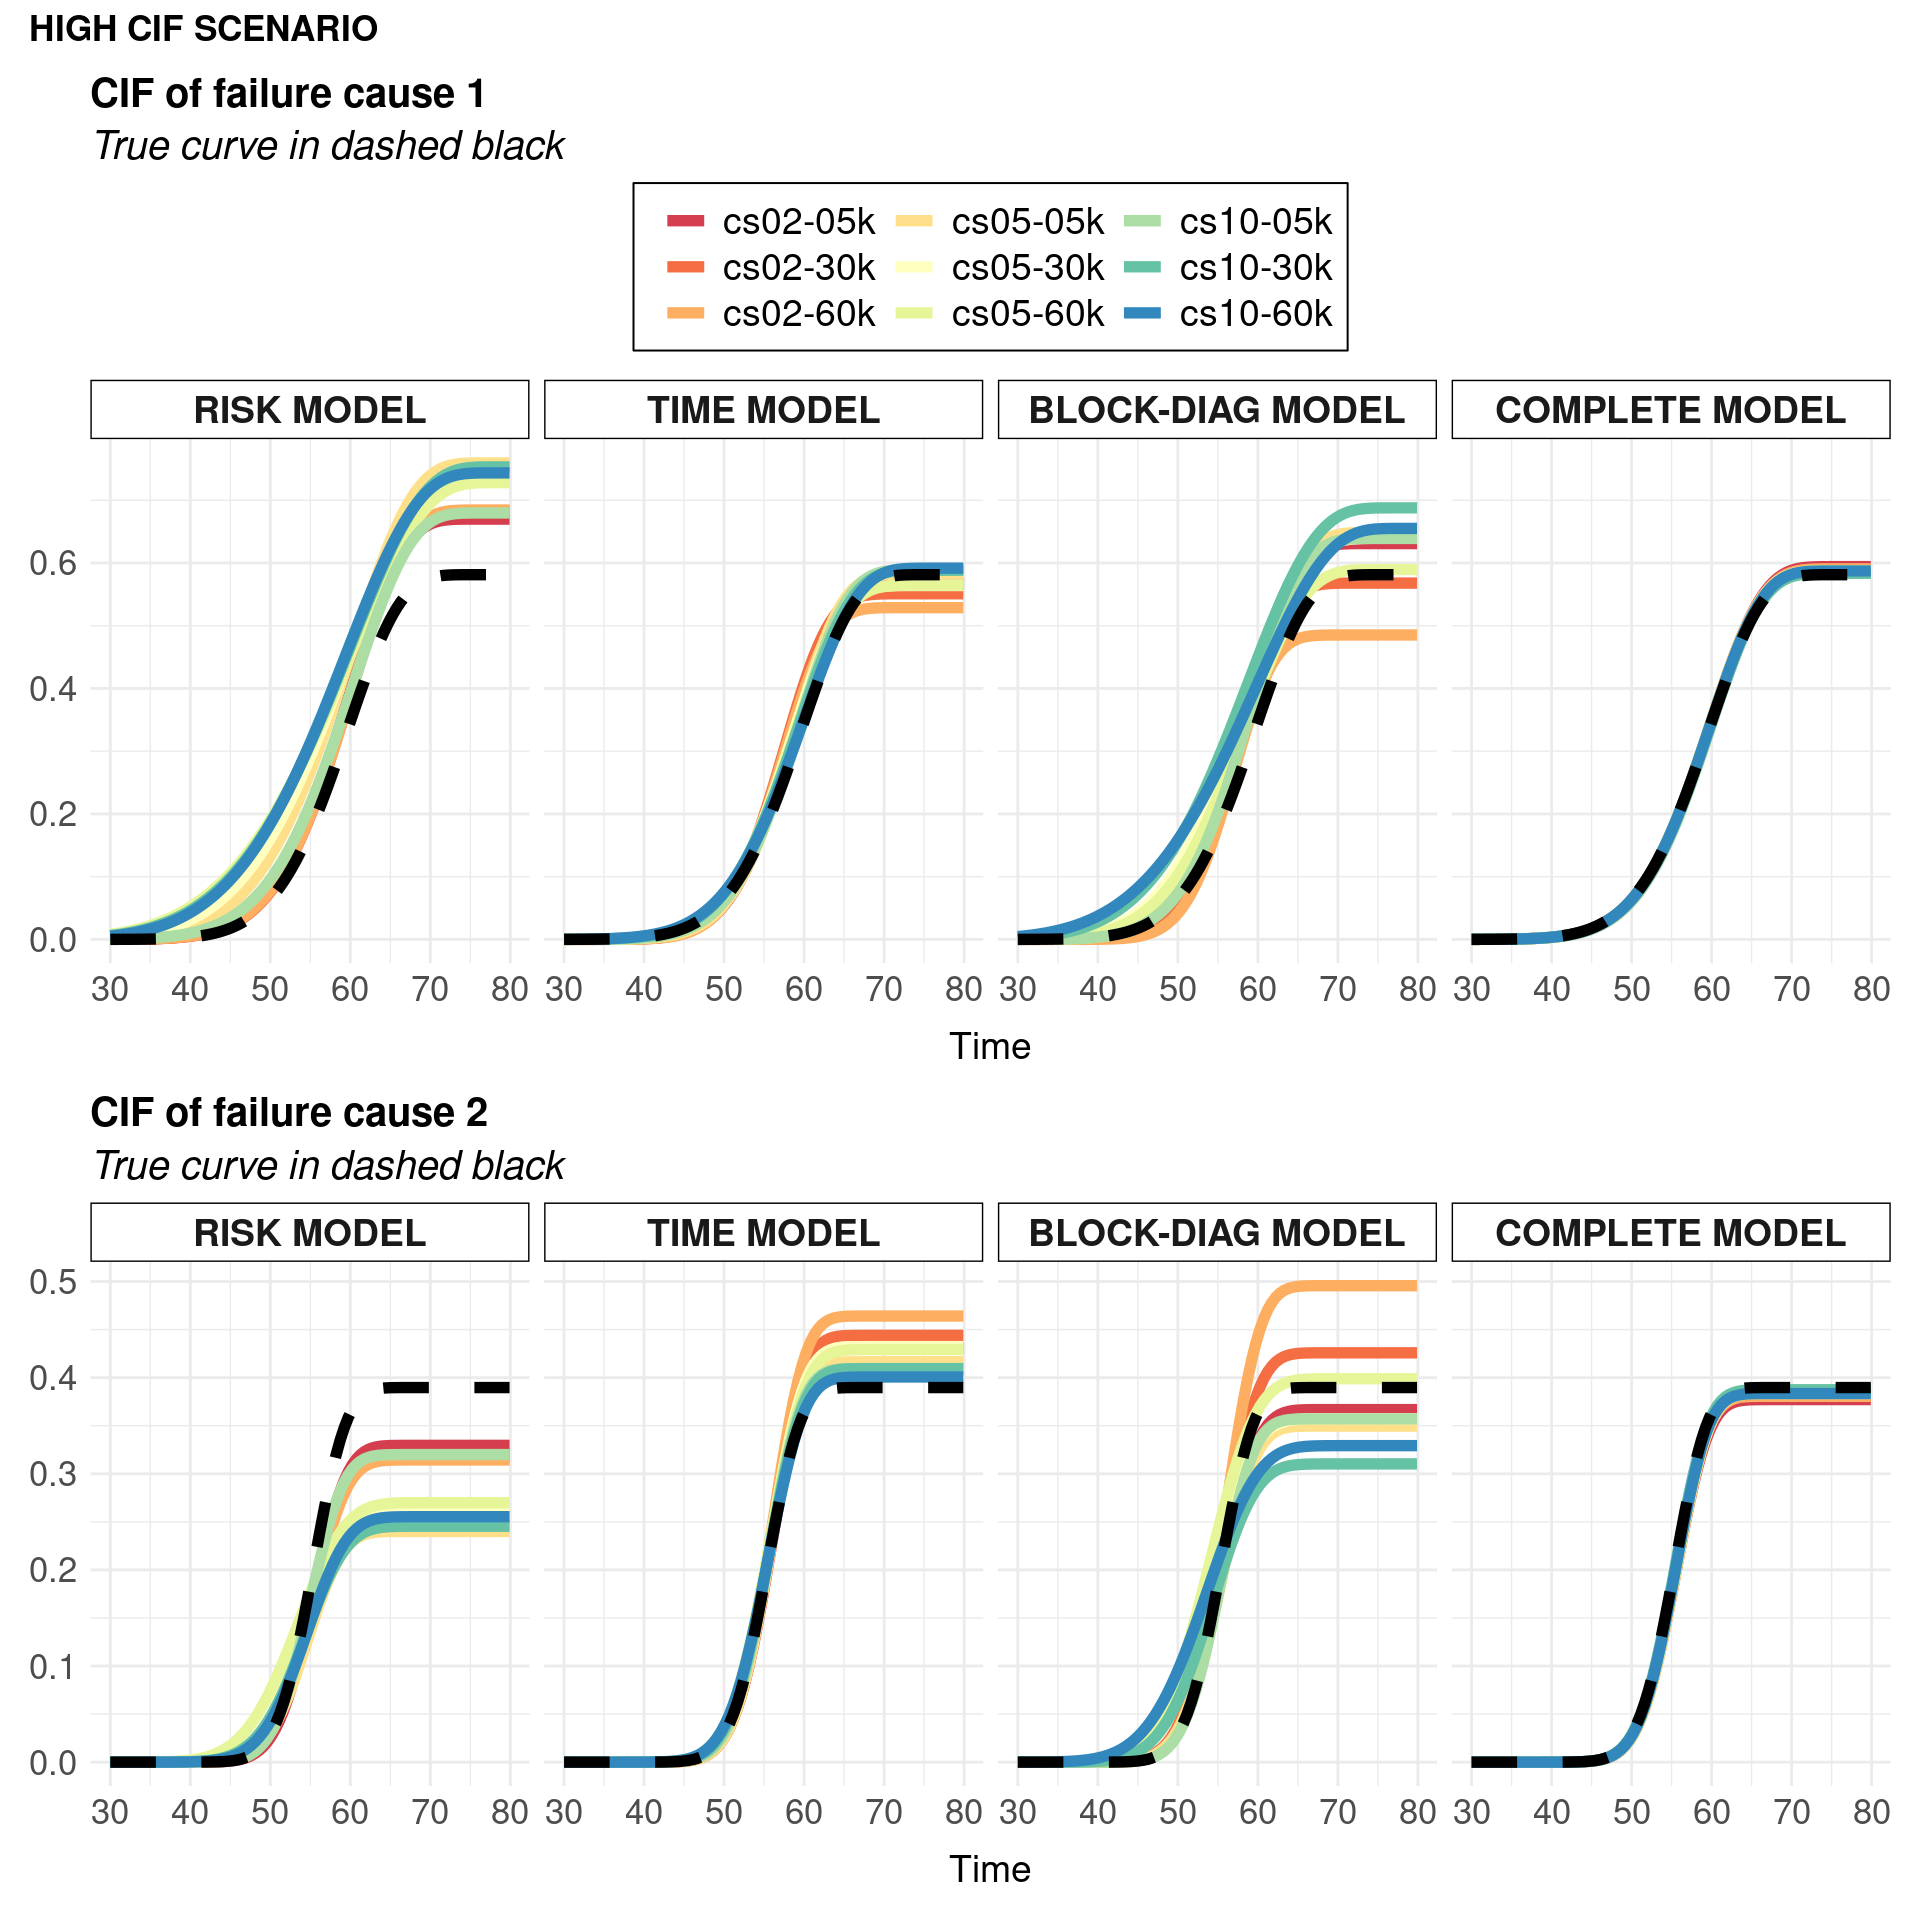
\includegraphics[width=\textwidth]{cifs-1.png}\\
%%  \begin{footnotesize}
%%   SOURCE: The author (2021).
%%  \end{footnotesize}
%%  \label{fig:cifs}
%% \end{figure}

% END ==================================================================
